\documentclass[12pt,a4paper]{article}

% ─── Packages ────────────────────────────────────────────────────────────────
\usepackage[a4paper, margin=1.5cm]{geometry}
\usepackage{fontenc}
\usepackage[utf8]{inputenc}
\usepackage{microtype}
\usepackage{xcolor}
\usepackage{graphicx}
\usepackage{amsmath,amssymb}
\usepackage{tcolorbox}
\usepackage{tikz}
\usetikzlibrary{arrows.meta, shapes.geometric, positioning, fit, backgrounds, calc}
\usepackage{mdframed}
\usepackage{booktabs}
\usepackage{array}
\usepackage{enumitem}
\usepackage{multicol}
\usepackage{fancyhdr}
\usepackage{titlesec}
\usepackage{graphicx}
\usepackage{subcaption}
% ─── Colours ─────────────────────────────────────────────────────────────────
\definecolor{deepblue}{HTML}{1A237E}
\definecolor{midblue}{HTML}{1565C0}
\definecolor{lightblue}{HTML}{E3F2FD}
\definecolor{accentorange}{HTML}{E65100}
\definecolor{accentyellow}{HTML}{FFF8E1}
\definecolor{successgreen}{HTML}{1B5E20}
\definecolor{lightgreen}{HTML}{E8F5E9}
\definecolor{warningyellow}{HTML}{F57F17}
\definecolor{lightgray}{HTML}{F5F5F5}
\definecolor{medgray}{HTML}{9E9E9E}
\definecolor{darkgray}{HTML}{424242}
\definecolor{alertred}{HTML}{B71C1C}
\definecolor{lightalert}{HTML}{FFEBEE}

% ─── Section formatting ───────────────────────────────────────────────────────
\titleformat{\section}{\large\bfseries\color{deepblue}}{}{0pt}{}[\color{midblue}\titlerule]
\titlespacing{\section}{0pt}{10pt}{5pt}
\setlength{\parindent}{0pt}
\setlength{\parskip}{4pt}

% ─── tcolorbox styles ────────────────────────────────────────────────────────
\tcbuselibrary{skins, breakable, listings}

\newtcolorbox{claimbox}[2][]{
  enhanced, breakable,
  colback=#2!8, colframe=#2!70!black,
  fonttitle=\bfseries\small, title=#1,
  boxrule=1pt, arc=4pt,
  left=6pt, right=6pt, top=4pt, bottom=4pt
}

\newtcolorbox{keybox}[1][]{
  enhanced,
  colback=accentyellow, colframe=accentorange,
  fonttitle=\bfseries\small, title=#1,
  boxrule=1.5pt, arc=4pt,
  left=6pt, right=6pt, top=4pt, bottom=4pt
}

\newtcolorbox{graybox}[1][]{
  enhanced,
  colback=lightgray, colframe=medgray,
  fonttitle=\bfseries\small, title=#1,
  boxrule=0.8pt, arc=4pt,
  left=6pt, right=6pt, top=4pt, bottom=4pt
}

% ─── Page style ───────────────────────────────────────────────────────────────
\pagestyle{fancy}
\fancyhf{}
\fancyhead[L]{\small\color{medgray}\textit{MVA 2025--2026 — CentraleSupélec}}
\fancyhead[R]{\small\color{medgray}\textit{Beruard \& Kapotos}}
\fancyfoot[C]{\small\color{medgray}\thepage}
\renewcommand{\headrulewidth}{0.3pt}
\renewcommand{\footrulewidth}{0pt}

% ─── Custom commands ─────────────────────────────────────────────────────────
\newcommand{\important}[1]{\textbf{\color{midblue}#1}}
\newcommand{\highlight}[1]{\colorbox{lightblue}{\strut #1}}
\newcommand{\bad}[1]{\textcolor{alertred}{#1}}
\newcommand{\good}[1]{\textcolor{successgreen}{#1}}
\newcommand{\placeholder}[1]{%
  \begin{center}
    \begin{tikzpicture}
      \node[draw=medgray, dashed, fill=lightgray, rounded corners=4pt,
            minimum width=\linewidth-10pt, minimum height=#1,
            text=darkgray, font=\small\itshape]
        {[Insert figure here]};
    \end{tikzpicture}
  \end{center}
}

\begin{document}

% ══════════════════════════════════════════════════════════════════════════════
%  PAGE 1 — TITLE + MOTIVATION + PAPER OVERVIEW
% ══════════════════════════════════════════════════════════════════════════════
% ─── Banner ──────────────────────────────────────────────────────────────────
\begin{tcolorbox}[
  enhanced, colback=deepblue, colframe=deepblue,
  arc=6pt, boxrule=0pt,
  left=12pt, right=12pt, top=10pt, bottom=10pt
]
  {\color{white}\Large\bfseries Small-Scale Proxies for Large-Scale\\[2pt]
   Transformer Training Instabilities}\\[6pt]
  {\color{lightblue}MVA 2025–2026}\\[4pt]
  {\color{white!70!deepblue}\small
   Tristan Beruard \& Fotios Kapotos\quad|\quad CentraleSupélec / MVA}
\end{tcolorbox}


\section*{Introduction}
\noindent
\begin{minipage}[t]{0.48\linewidth}
\begin{claimbox}[Why This Matters]{alertred}
\small
\textbf{Large Transformer training is expensive.}

When a billion-scale run diverges, you lose compute, time, and signal.

\medskip
\textit{Worse: failures do not reproduce at small scale.}

Debugging becomes guesswork.
\end{claimbox}
\end{minipage}
\hfill
\begin{minipage}[t]{0.48\linewidth}
\begin{claimbox}[Key Insight]{successgreen}
\small
\textbf{High learning rates mimic large scale.}

Push a small model into extreme LR →
same instabilities appear.

\medskip
\textit{Result: failures become cheap to reproduce, study, and fix.}
\end{claimbox}
\end{minipage}

\vspace{6pt}
\section{Paper Overview}
\noindent
\begin{minipage}[t]{0.32\linewidth}
\begin{graybox}[Step 1: Identify, equal height group=A]
\small
Two failure modes from large-scale runs:
\begin{itemize}[leftmargin=12pt, itemsep=1pt]
  \item Attention logit growth
  \item Output logit divergence
\end{itemize}
Reproduced in small models at high LR.
\end{graybox}
\end{minipage}
\hfill
\begin{minipage}[t]{0.32\linewidth}
\begin{graybox}[Step 2: Mitigate, equal height group=A]
\small
Test proposed fixes:
\begin{itemize}[leftmargin=12pt, itemsep=1pt]
  \item \textbf{qk-layernorm}: normalize Q,K
  \item \textbf{z-loss}: penalty $\alpha \log^2 Z$
\end{itemize}
\end{graybox}
\end{minipage}
\hfill
\begin{minipage}[t]{0.32\linewidth}
\begin{graybox}[Step 3: Quantify, equal height group=A]
\small
Define LR sensitivity $\mathcal{S}$:
\[
\mathcal{S} = \mathbb{E}_{\eta\in[a,b]}\!\bigl[\min(\ell(A(\eta)),\ell_0) - \ell^*\bigr]
\]

How much performance drops under bad LR.

High $\mathcal{S}$ = fragile.
\end{graybox}
\end{minipage}

\section{Methodology}

\begin{graybox}[Experimental setup \& training]
\small
\begin{itemize}[leftmargin=12pt, itemsep=2pt]
  \item Decoder-only Transformer based on nanoGPT
  \item Architecture close to the paper: rotary embeddings, no dropout, bias-free layers
  \item \textbf{Next-token prediction} on OpenWebText-style dataset
  \item Training with \textbf{AdamW} (\(\beta_1=0.9\), \(\beta_2=0.95\)), batch size \(32\), sequence length \(256\), bf16
\end{itemize}
\end{graybox}


\section{Claims}

\begin{tcolorbox}[
  colback=lightblue,
  colframe=midblue,
  boxrule=0.8pt,
  arc=4pt,
  title=\textbf{Claim 1}
]
\small
The queries and keys in self-attention layers grow unboundedly, causing the softmax to collapse to a one-hot distribution and learning to stall. The proposed fix is \emph{qk-layernorm}, which applies LayerNorm t queries and keys before the dot product.
\end{tcolorbox}
\begin{tcolorbox}[
  colback=accentyellow,
  colframe=accentorange,
  boxrule=0.8pt,
  arc=4pt,
  title=\textbf{Claim 2}
]
\small
The output logits drift to very negative values, decoupling them from the log probabilities.
\end{tcolorbox}
\newpage
% ══════════════════════════════════════════════════════════════════════════════
%  PAGE 2 — INSTABILITY 1: ATTENTION LOGIT GROWTH
% ══════════════════════════════════════════════════════════════════════════════

\begin{tcolorbox}[
  enhanced, colback=midblue!15, colframe=midblue,
  arc=6pt, boxrule=1.5pt, left=10pt, right=10pt, top=6pt, bottom=6pt
]
  {\large\bfseries\color{deepblue} Instability \#1 — Attention Logit Growth}
\end{tcolorbox}

\vspace{8pt}

\begin{multicols}{2}

\section{Mechanism}

In self-attention, the logit between position $i$ and $j$ in a head of dimension $d_h$ is:
\[
z_{ij} = \frac{\langle q_i,\, k_j\rangle}{\sqrt{d_h}}
\]
Both $q_i$ and $k_j$ grow linearly with their weight matrix norms, so $z_{ij}$ grows
\textbf{quadratically} with parameter norm — \important{much faster} than any other quantity
in the network.

\medskip
\begin{claimbox}[What happens next]{alertred}
\small
Once logits are very large, the softmax collapses to a \textbf{one-hot distribution}:
every token attends to a single fixed position regardless of content.
The attention mechanism becomes \emph{content-independent} and learning stalls.
\end{claimbox}
\columnbreak

\section{The Fix — qk-LayerNorm}

\begin{center}
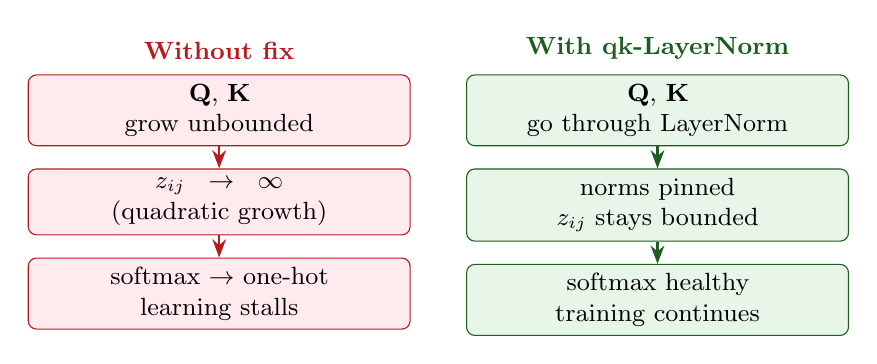
\begin{tikzpicture}[font=\small, node distance=8pt, >=Stealth]
  % Without
  \node[draw=alertred, fill=lightalert, rounded corners=3pt,
        minimum width=0.4\linewidth, text width=0.38\linewidth,
        align=center, minimum height=20pt] (wq) {\textbf{Q}, \textbf{K}\\grow unbounded};
  \node[draw=alertred, fill=lightalert, rounded corners=3pt,
        minimum width=0.4\linewidth, text width=0.38\linewidth,
        align=center, minimum height=20pt, below=of wq] (wz) {$z_{ij} \to \infty$\\(quadratic growth)};
  \node[draw=alertred, fill=lightalert, rounded corners=3pt,
        minimum width=0.4\linewidth, text width=0.38\linewidth,
        align=center, minimum height=20pt, below=of wz] (wc) {softmax $\to$ one-hot\\learning stalls};
  \draw[->, alertred, thick] (wq)--(wz);
  \draw[->, alertred, thick] (wz)--(wc);
  \node[above=2pt of wq, color=alertred, font=\bfseries\small] {Without fix};

  % With
  \node[draw=successgreen, fill=lightgreen, rounded corners=3pt,
        minimum width=0.4\linewidth, text width=0.38\linewidth,
        align=center, minimum height=20pt, right=20pt of wq] (gq)
        {\textbf{Q}, \textbf{K}\\go through LayerNorm};
  \node[draw=successgreen, fill=lightgreen, rounded corners=3pt,
        minimum width=0.4\linewidth, text width=0.38\linewidth,
        align=center, minimum height=20pt, below=of gq] (gz)
        {norms pinned\\$z_{ij}$ stays bounded};
  \node[draw=successgreen, fill=lightgreen, rounded corners=3pt,
        minimum width=0.4\linewidth, text width=0.38\linewidth,
        align=center, minimum height=20pt, below=of gz] (gc)
        {softmax healthy\\training continues};
  \draw[->, successgreen, thick] (gq)--(gz);
  \draw[->, successgreen, thick] (gz)--(gc);
  \node[above=2pt of gq, color=successgreen, font=\bfseries\small] {With qk-LayerNorm};
\end{tikzpicture}
\end{center}

\begin{claimbox}[Mitigation]{successgreen}
\small
\textbf{qk-LayerNorm}: apply LayerNorm to $q$ and $k$ \emph{before} computing the dot
product. This pins their norms, \textbf{breaking the quadratic dependence} on parameter norm.
The instability is completely prevented.
\end{claimbox}

\end{multicols}

\vspace{6pt}
\section{Claim 1 — Curves}

\begin{minipage}{\linewidth}
    \centering
    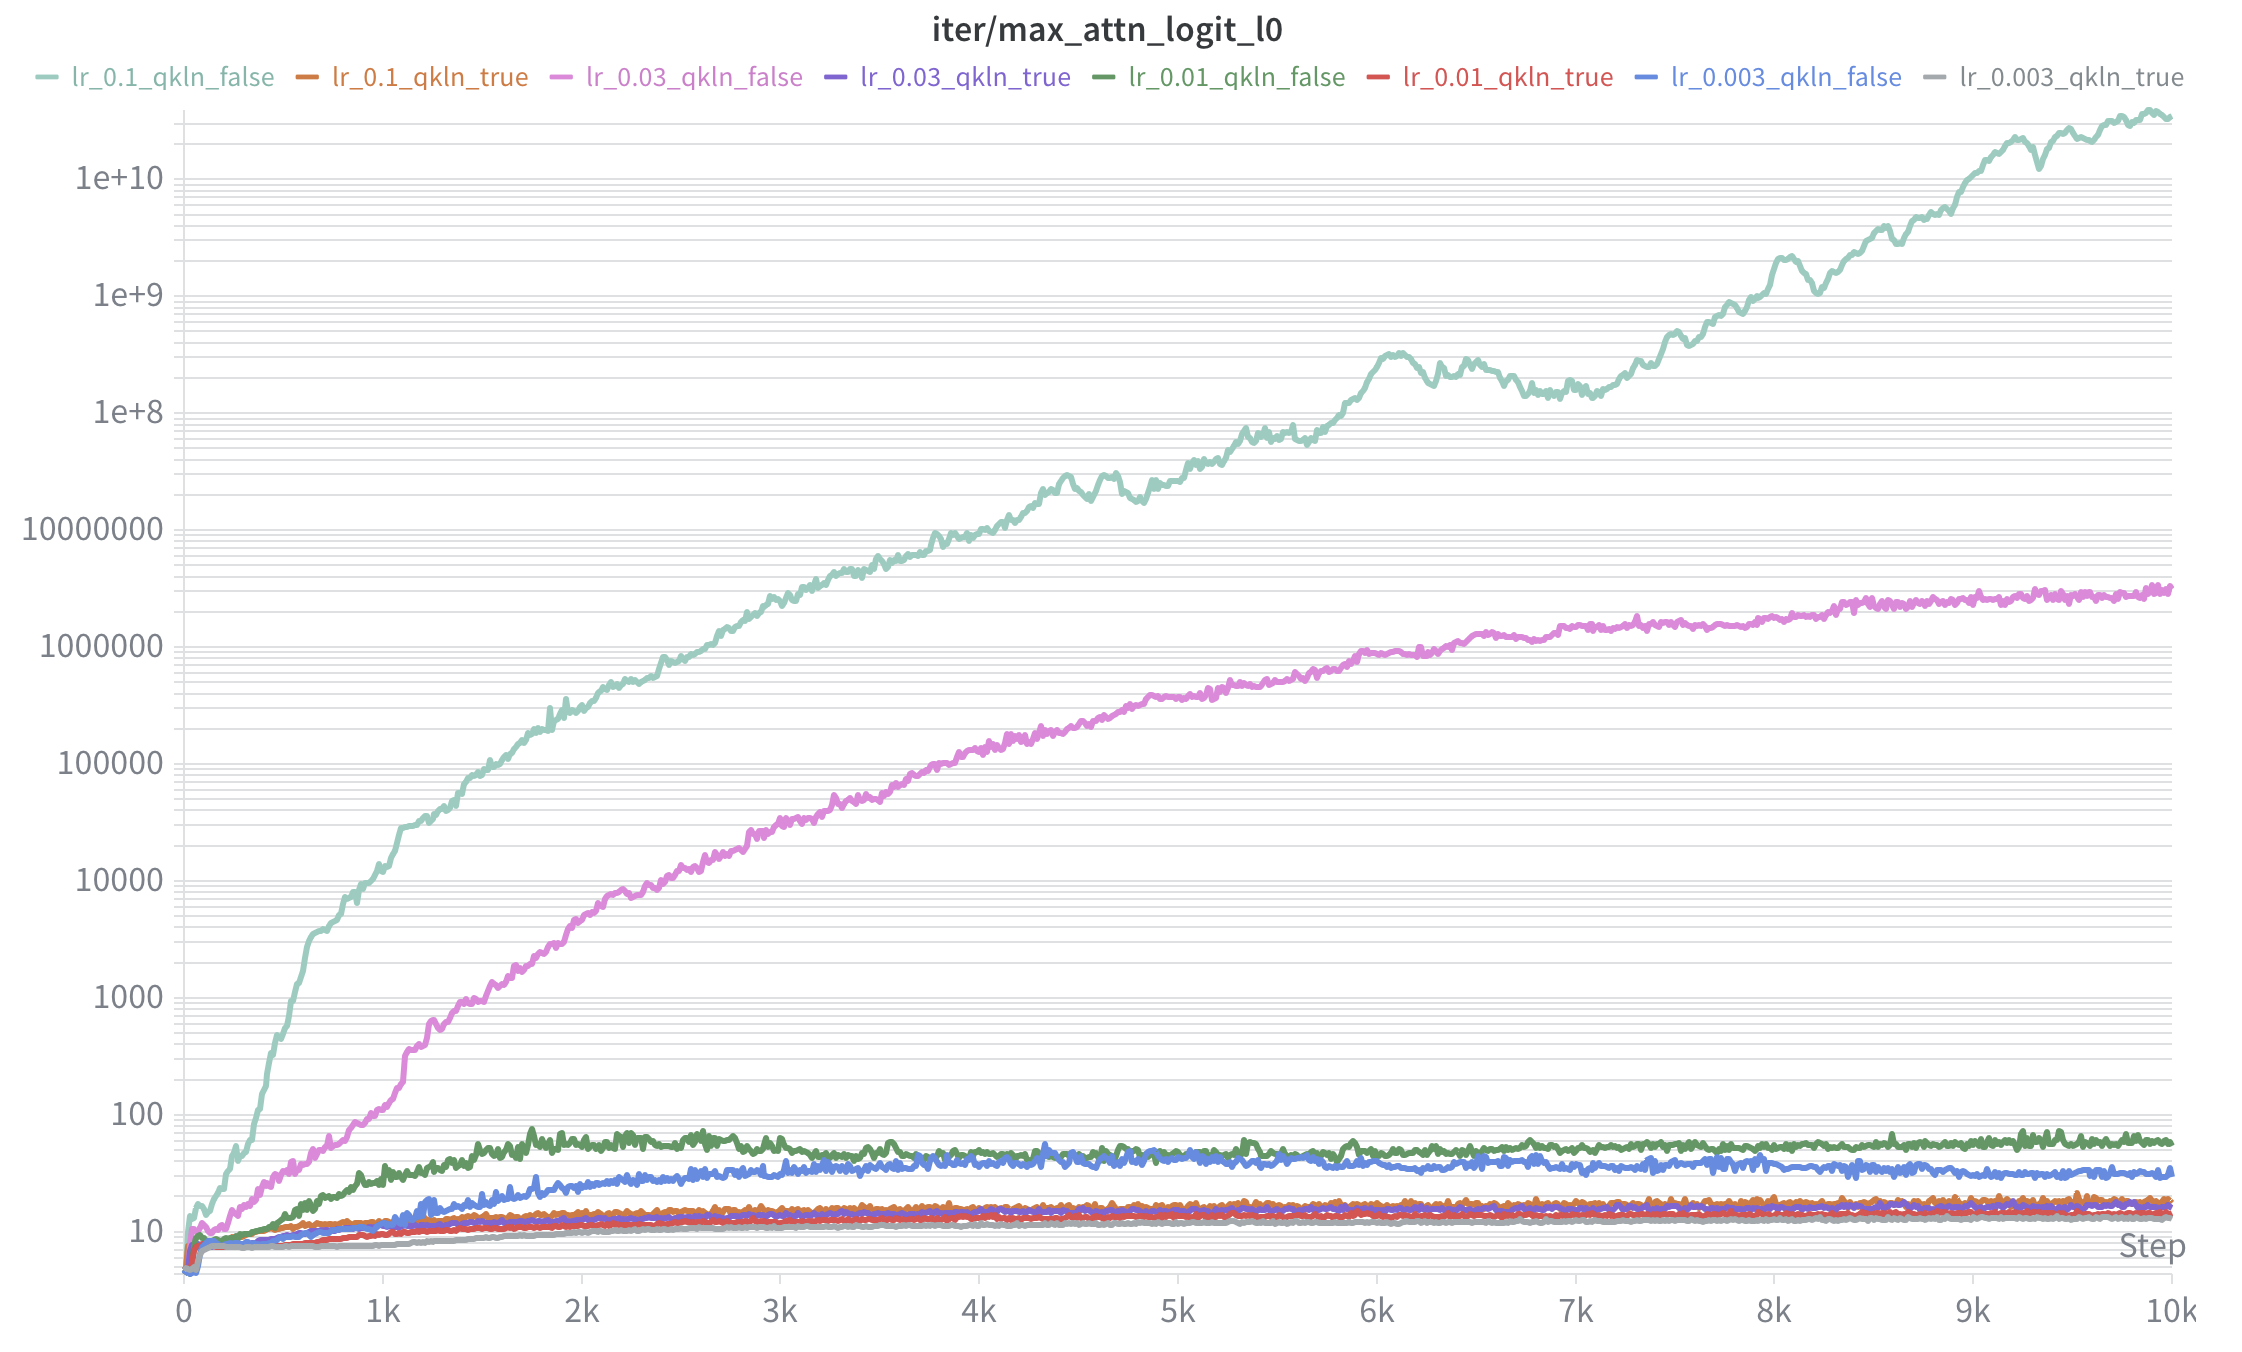
\includegraphics[width=0.9\linewidth]{../rapport/figures/C1_max_attn_logits.png}
    
    {\footnotesize Maximum attention logit over training. Divergence appears at high learning rates without qk-layernorm.}
\end{minipage}

\vspace{4pt}

\begin{minipage}{0.48\linewidth}
    \centering
    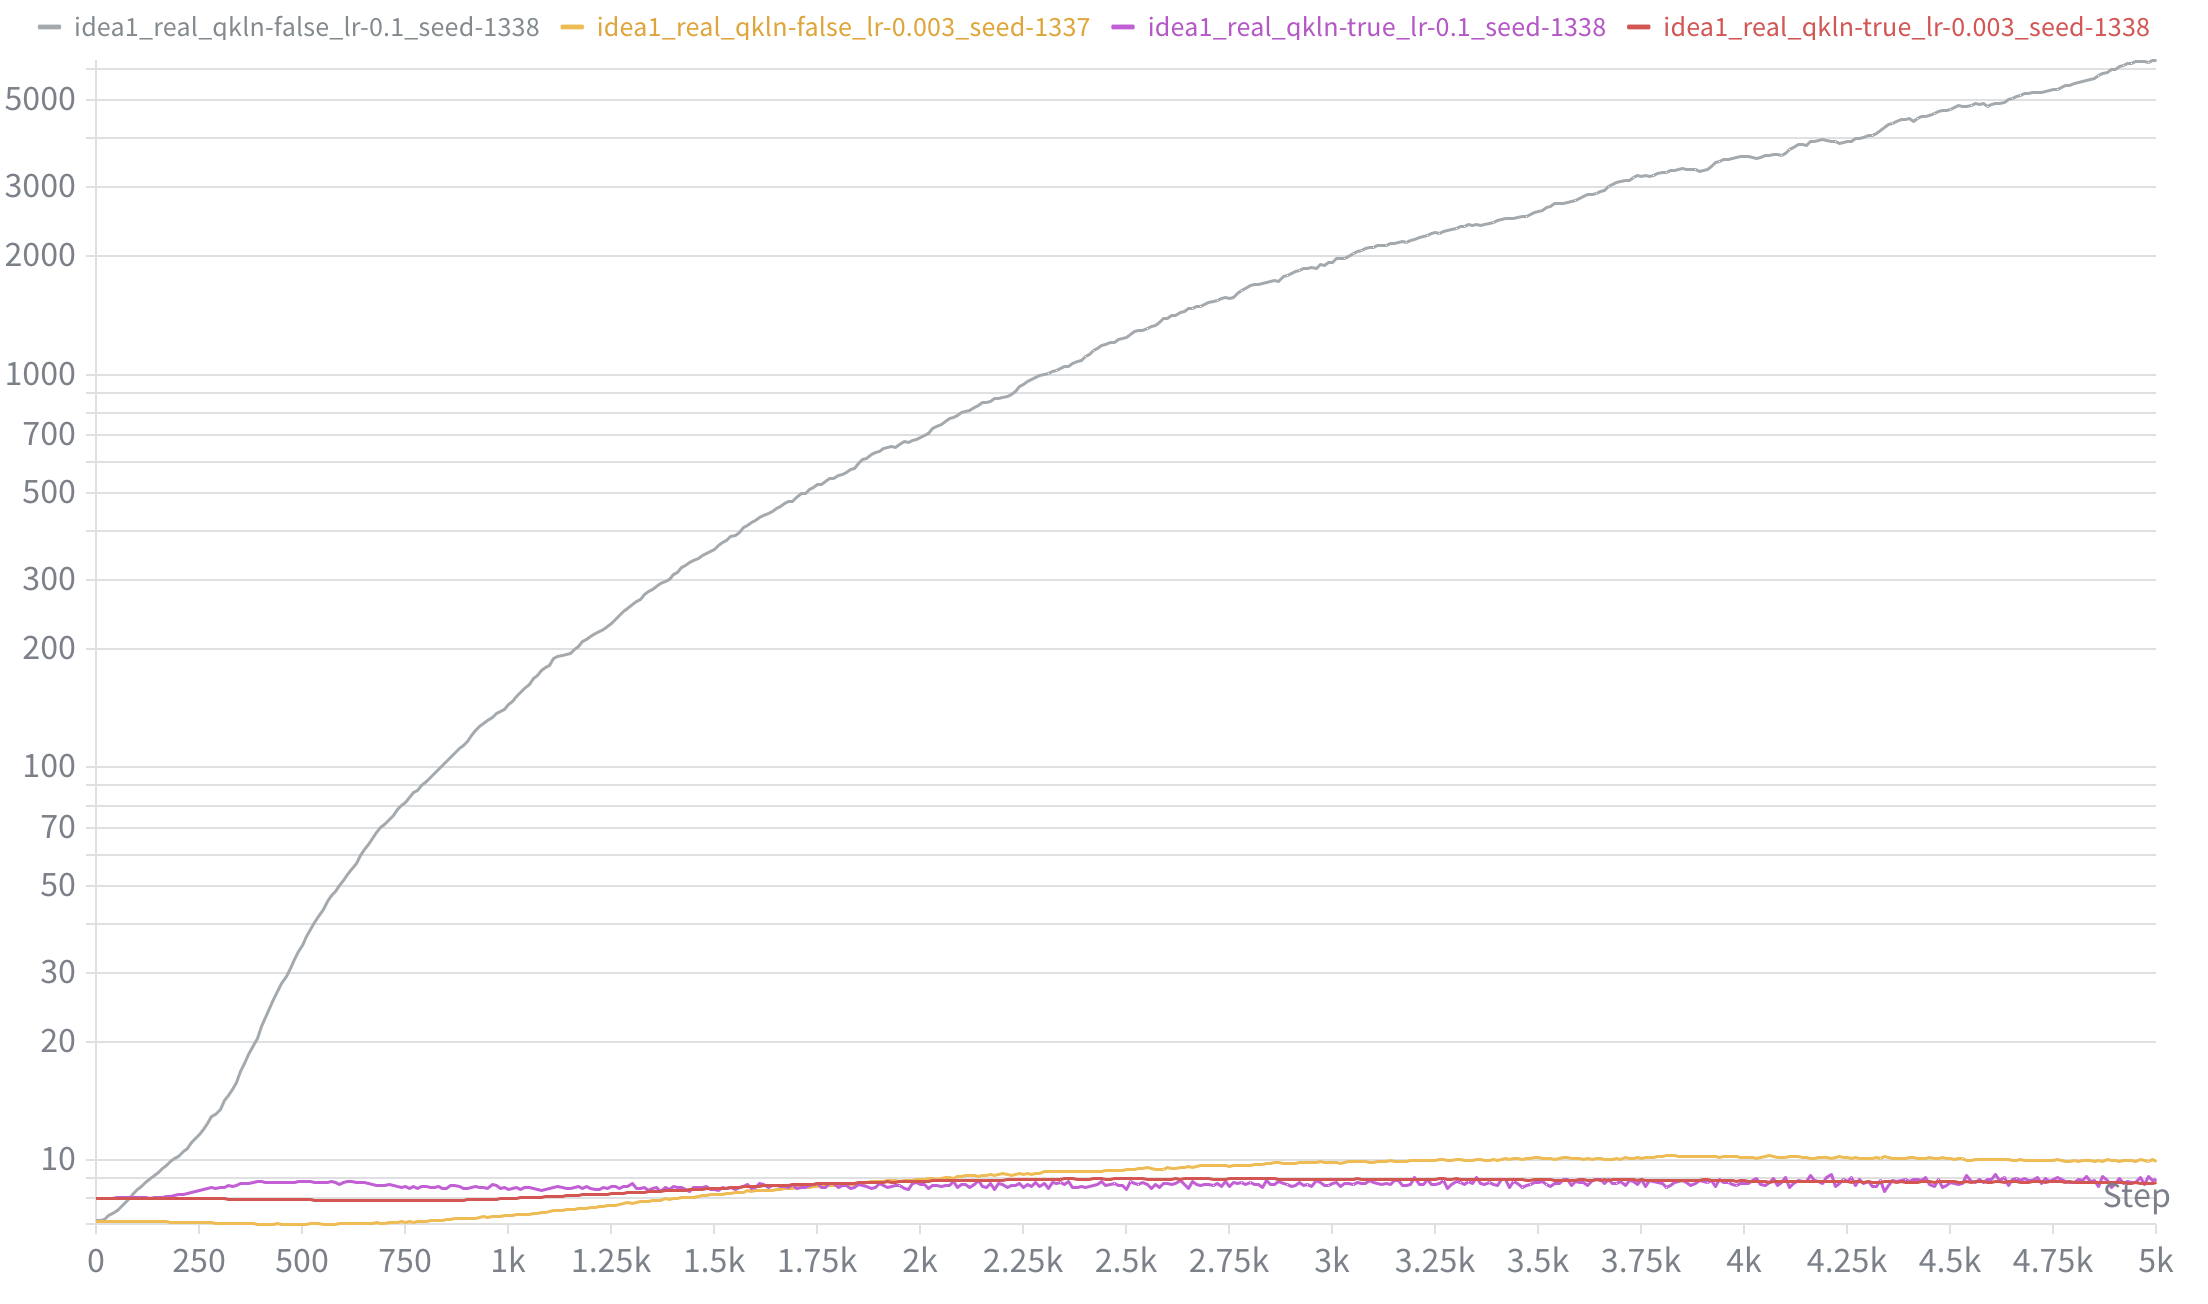
\includegraphics[width=\linewidth]{../rapport/figures/C1_qnorm.png}
    
    {\footnotesize Mean query norm}
\end{minipage}
\hfill
\begin{minipage}{0.48\linewidth}
    \centering
    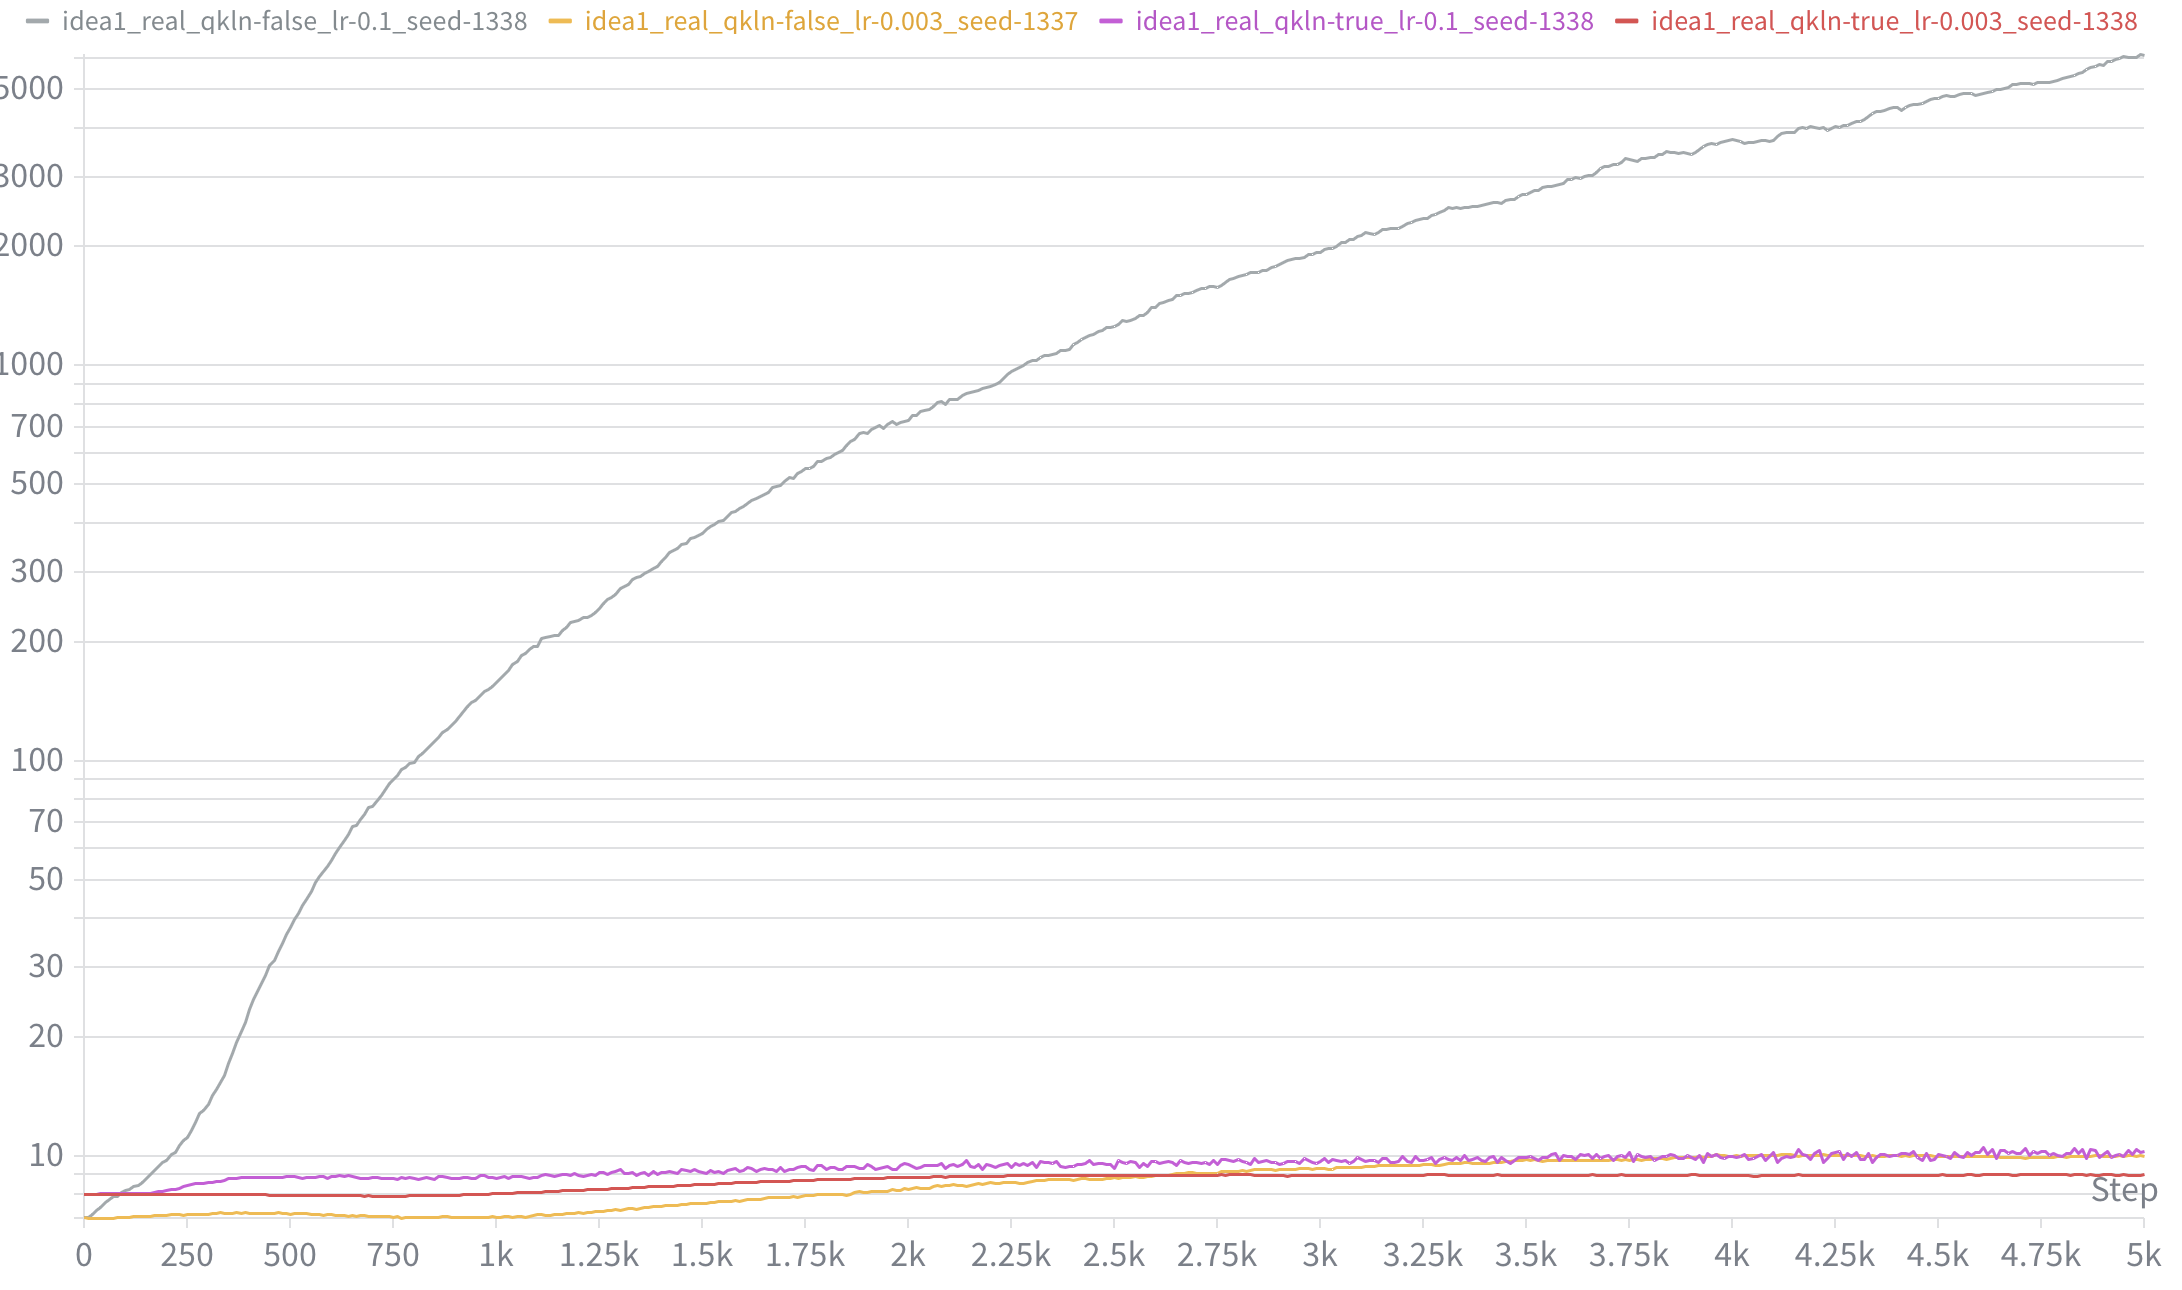
\includegraphics[width=\linewidth]{../rapport/figures/C1_knorm.png}
    
    {\footnotesize Mean key norm}
\end{minipage}

\vspace{4pt}

\begin{minipage}{0.48\linewidth}
    \centering
    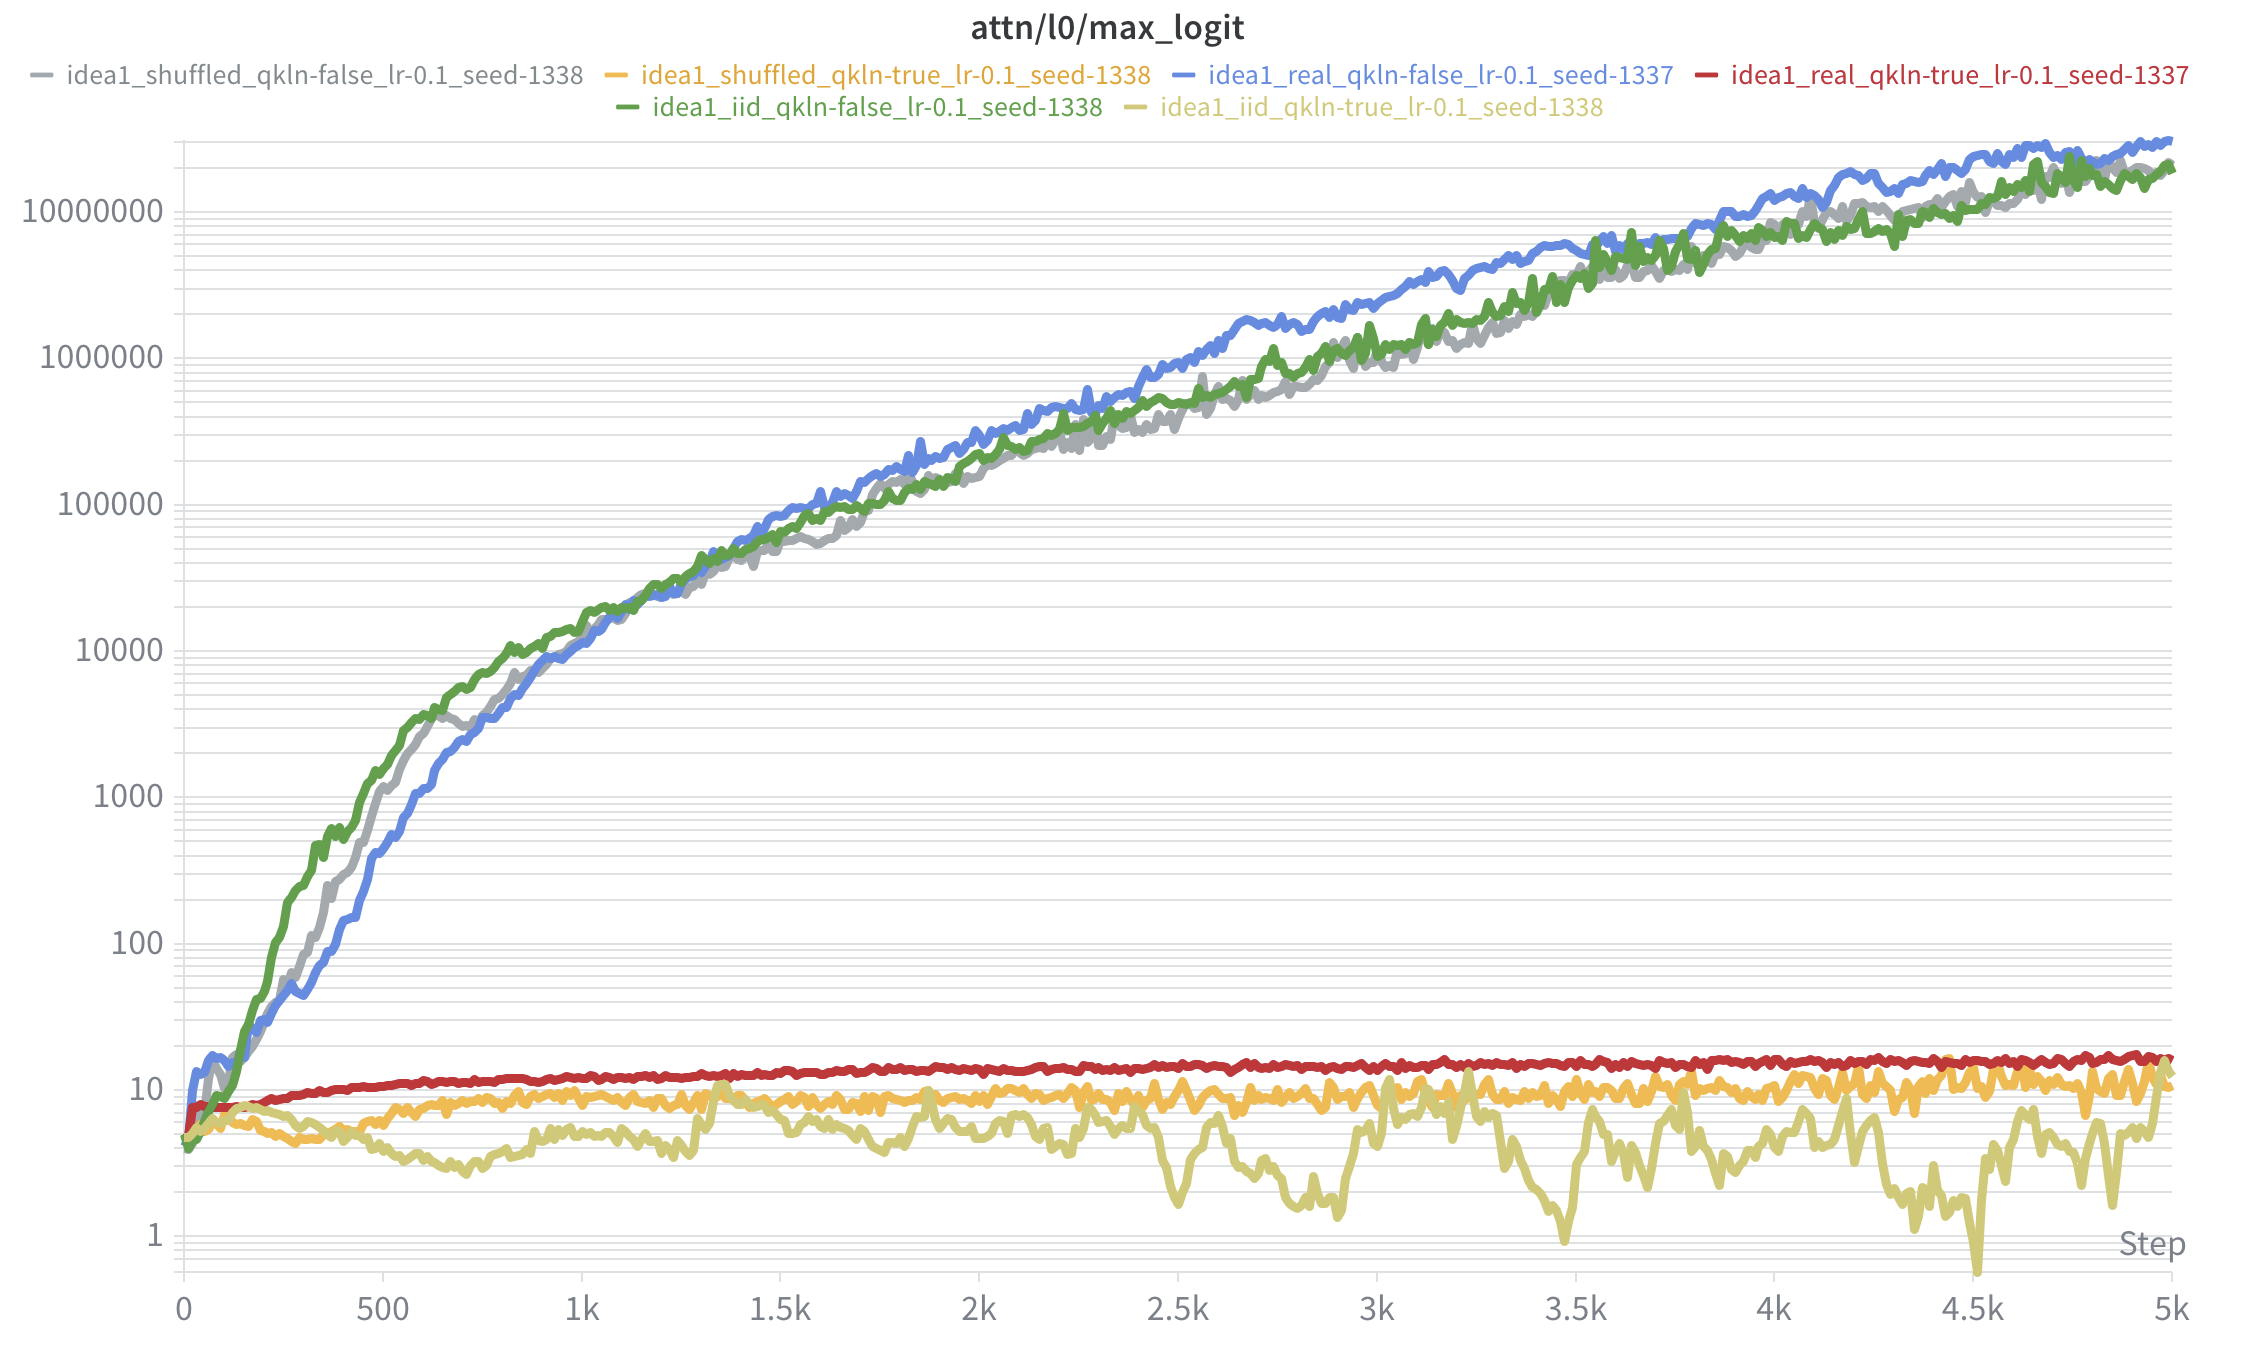
\includegraphics[width=\linewidth]{../rapport/figures/C1_multiple_data.png}
    
    {\footnotesize Max logits across datasets}
\end{minipage}
\hfill
\begin{minipage}{0.48\linewidth}
    \centering
    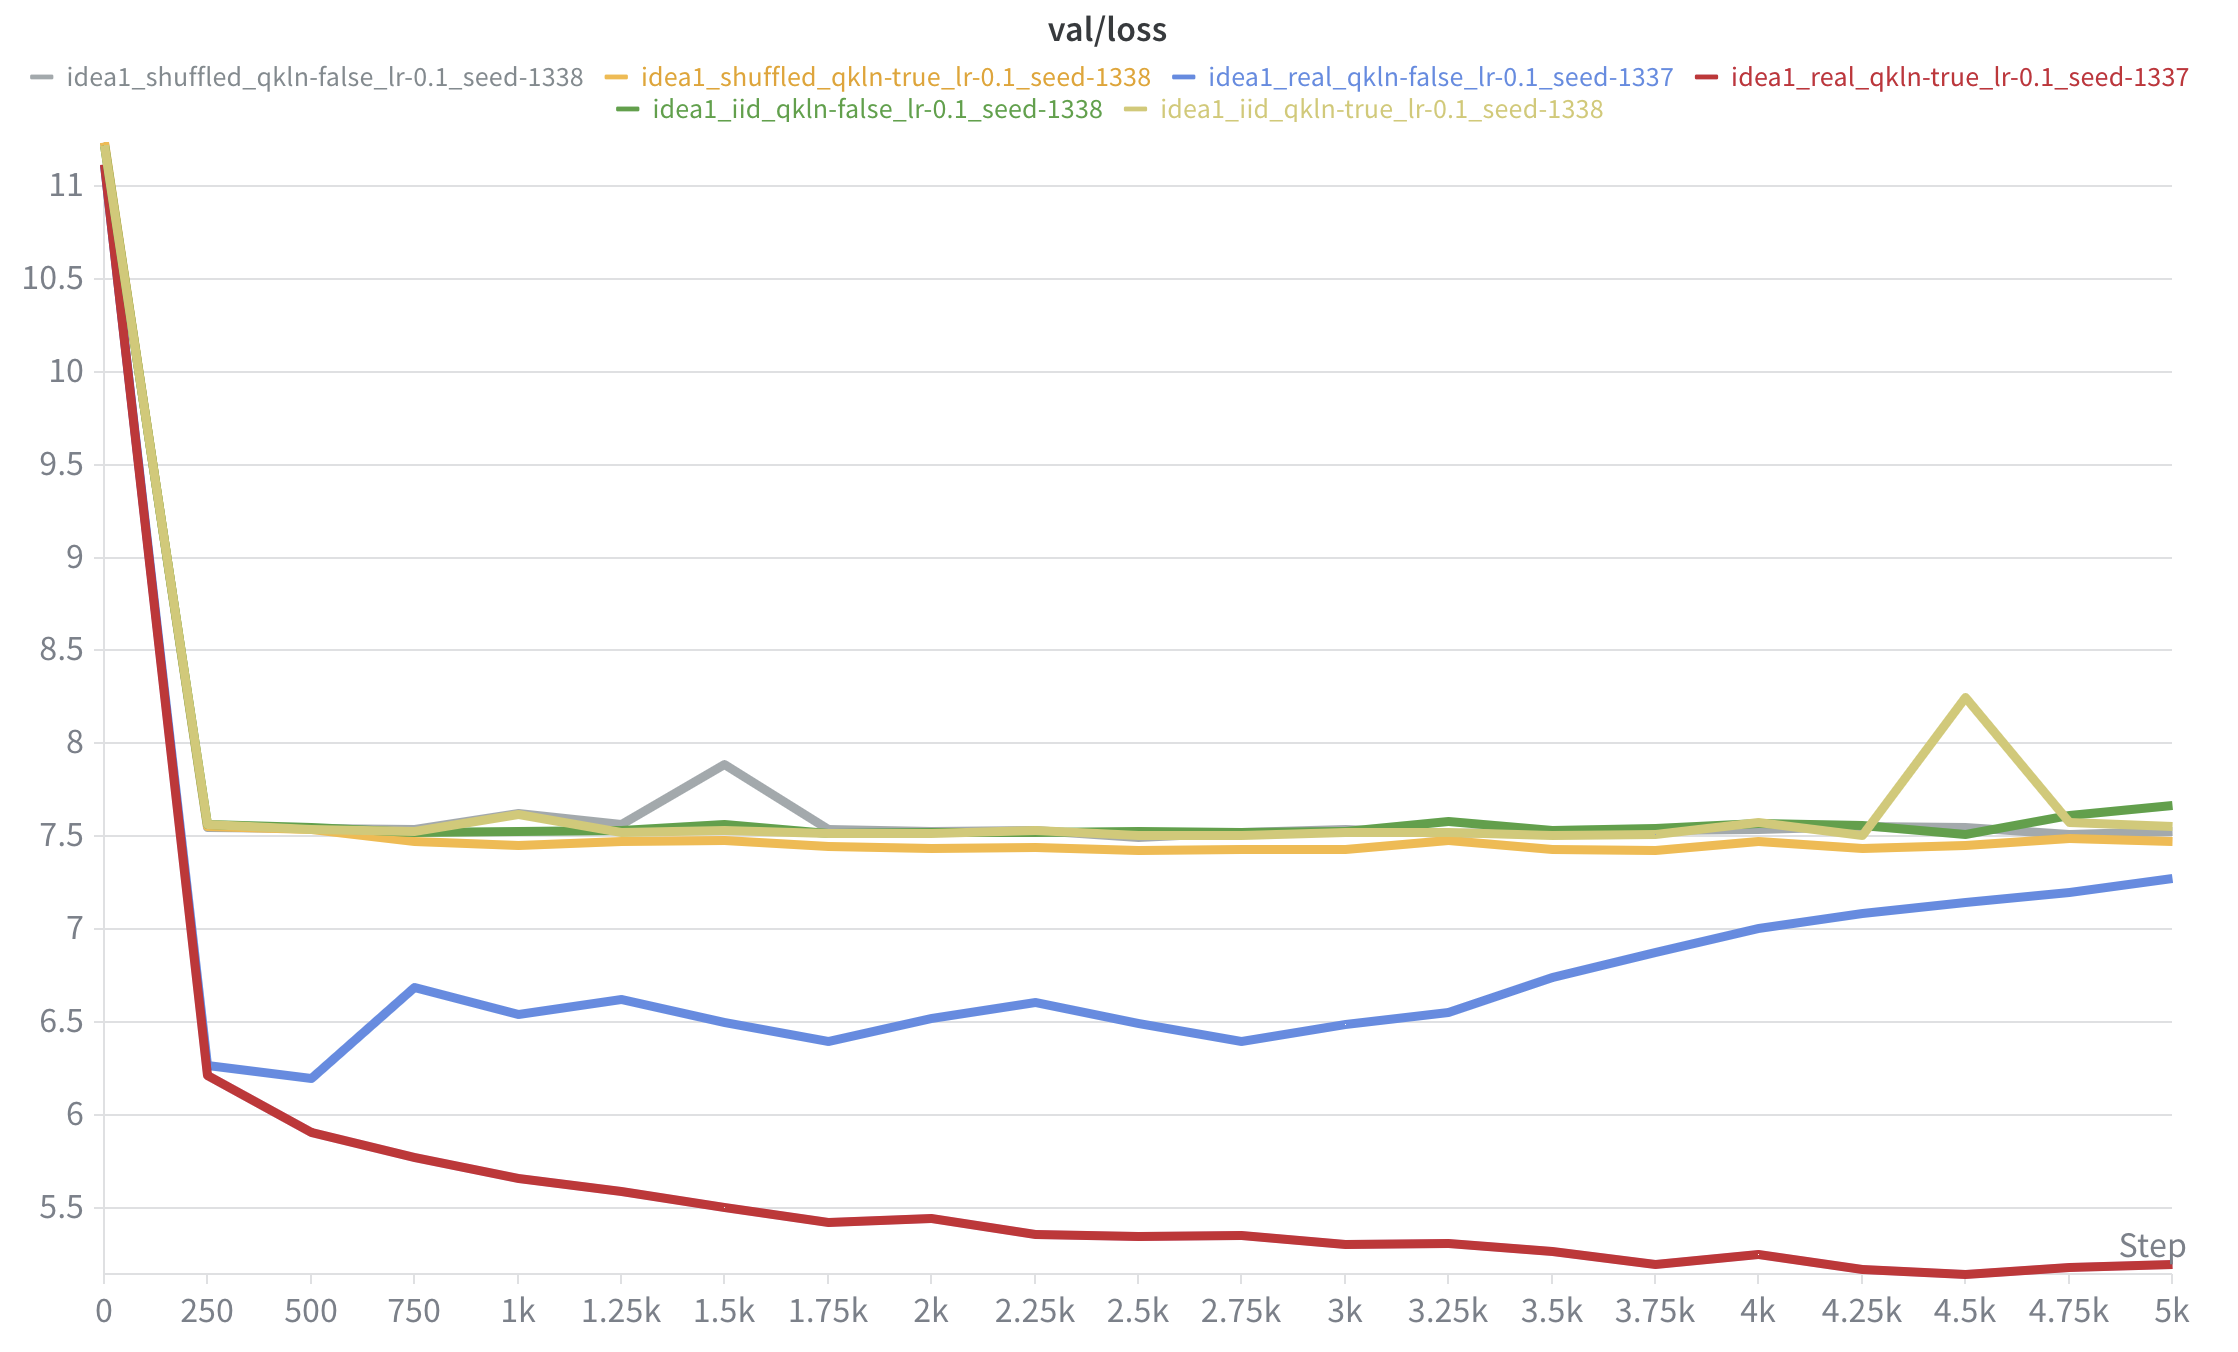
\includegraphics[width=\linewidth]{../rapport/figures/C1_losses_datasets.png}
    
    {\footnotesize Validation loss across datasets}
\end{minipage}

{\footnotesize
\textbf{Top:} Attention logit divergence appears at high learning rates when qk-layernorm is disabled. 
\textbf{Middle:} The norms of queries and keys increase sharply before divergence, indicating that the instability is driven by norm growth rather than improved alignment. 
\textbf{Bottom:} The same behavior is observed on standard, shuffled, and IID datasets, supporting the claim that the instability is optimizer-driven rather than data-dependent.
}
\newpage

% ══════════════════════════════════════════════════════════════════════════════
%  PAGE 3 — INSTABILITY 2: OUTPUT LOGIT DIVERGENCE
% ══════════════════════════════════════════════════════════════════════════════

\begin{tcolorbox}[
  enhanced, colback=accentorange!15, colframe=accentorange,
  arc=6pt, boxrule=1.5pt, left=10pt, right=10pt, top=6pt, bottom=6pt
]
  {\large\bfseries\color{accentorange} Instability \#2 — Output Logit Divergence}
\end{tcolorbox}

\vspace{8pt}

\begin{multicols}{2}

\section{Mechanism}

Let $y \in \mathbb{R}^V$ be the output logits, giving token probabilities:
\[
p_i = \frac{e^{y_i}}{Z}, \qquad Z = \sum_j e^{y_j}
\]
Without weight decay, the logits collectively drift toward \textbf{very negative values}
late in training.
This is distinct from attention logit growth: the divergence occurs
\emph{towards the end} of training, is \emph{global} (all logits shift), and only
manifests when \textbf{weight decay is absent}.

\columnbreak

\section{The Fix — Z-loss Regularisation}

The proposed mitigation (Chowdhery et al., 2022) is an auxiliary loss term:
\[
\mathcal{L}_{\text{z-loss}} = \alpha \log^2 Z, \qquad \alpha = 10^{-4}
\]

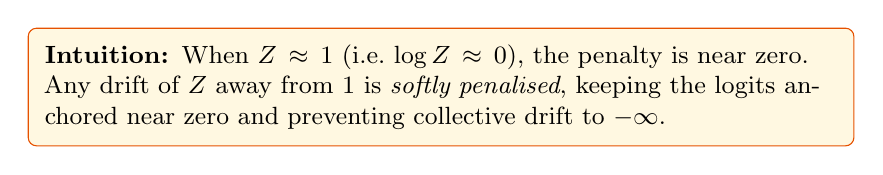
\begin{tikzpicture}[font=\small, >=Stealth, node distance=6pt]
  \node[draw=accentorange, fill=accentyellow, rounded corners=3pt,
        minimum width=0.85\linewidth, text width=0.83\linewidth,
        align=left, minimum height=16pt, inner sep=6pt] (intuition) {
    \textbf{Intuition:} When $Z \approx 1$ (i.e.\ $\log Z \approx 0$), the penalty is
    near zero. Any drift of $Z$ away from 1 is \emph{softly penalised}, keeping
    the logits anchored near zero and preventing collective drift to $-\infty$.
  };
\end{tikzpicture}

\end{multicols}

\vspace{6pt}
\section{Claim 2 — Curves}
\begin{minipage}{0.48\linewidth}
    \centering
    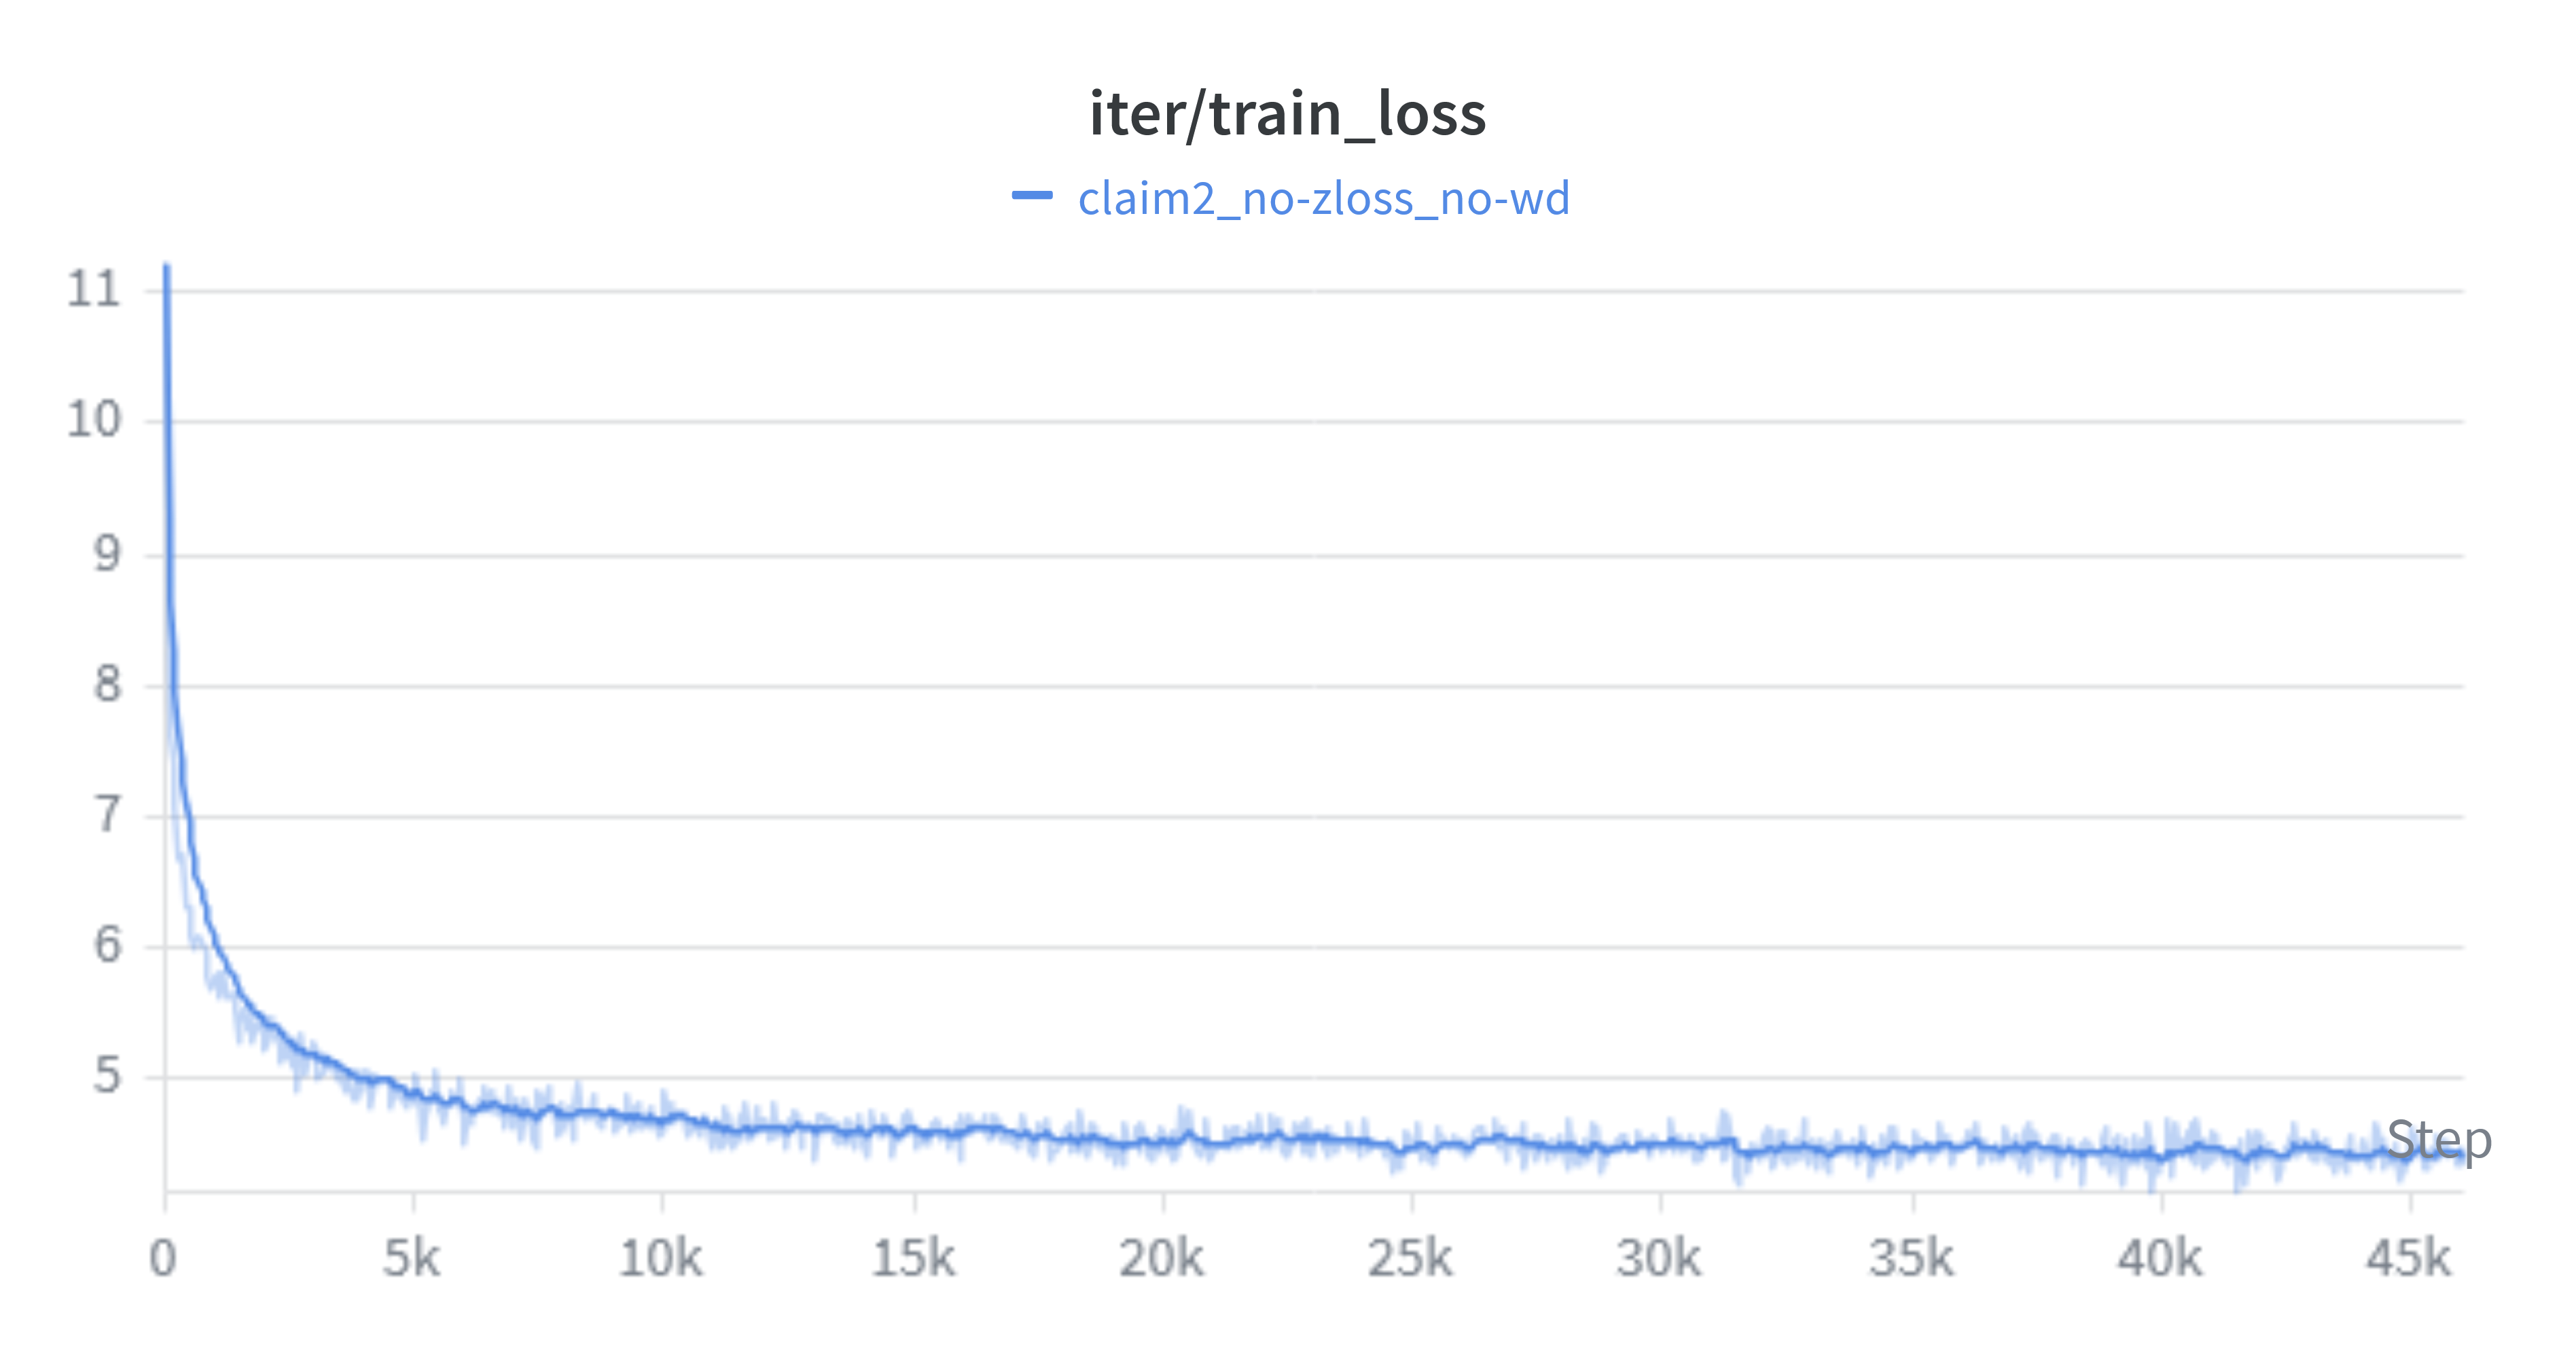
\includegraphics[width=\linewidth]{../rapport/figures/C2_train_loss_stable.png}
\end{minipage}
\hfill
\begin{minipage}{0.48\linewidth}
    \centering
    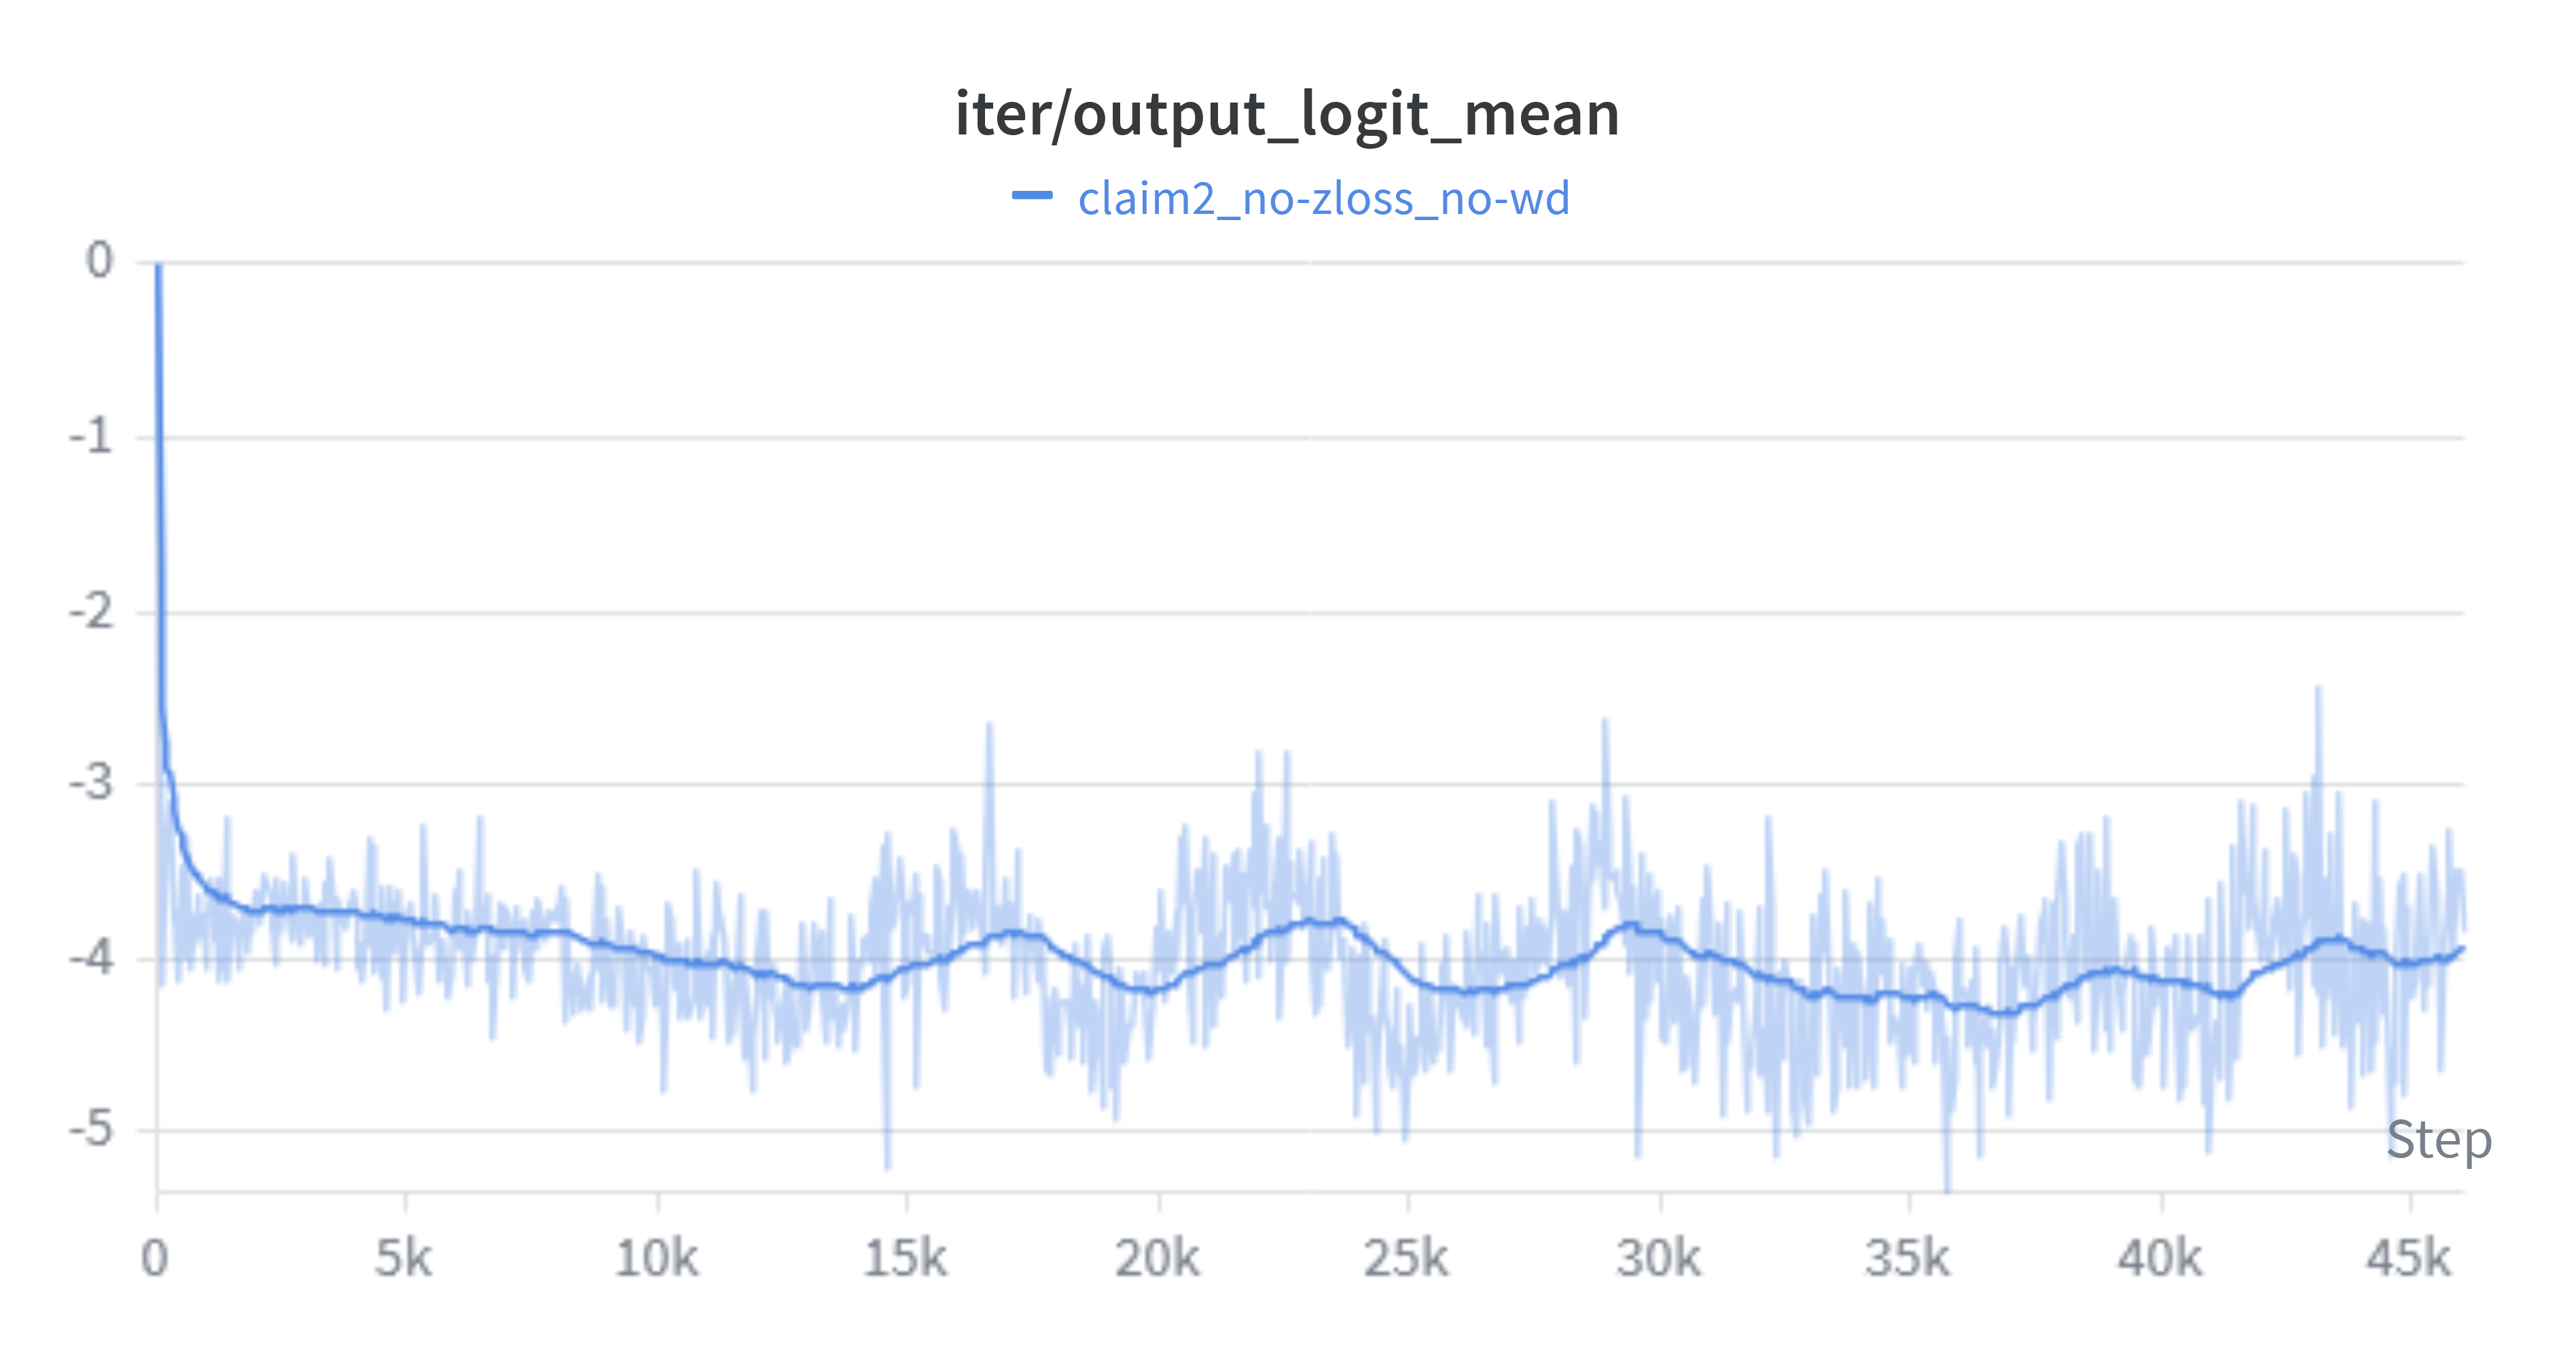
\includegraphics[width=\linewidth]{../rapport/figures/C2_logit_mean_stable.png}
\end{minipage}
\begin{minipage}{0.48\linewidth}
    \centering
    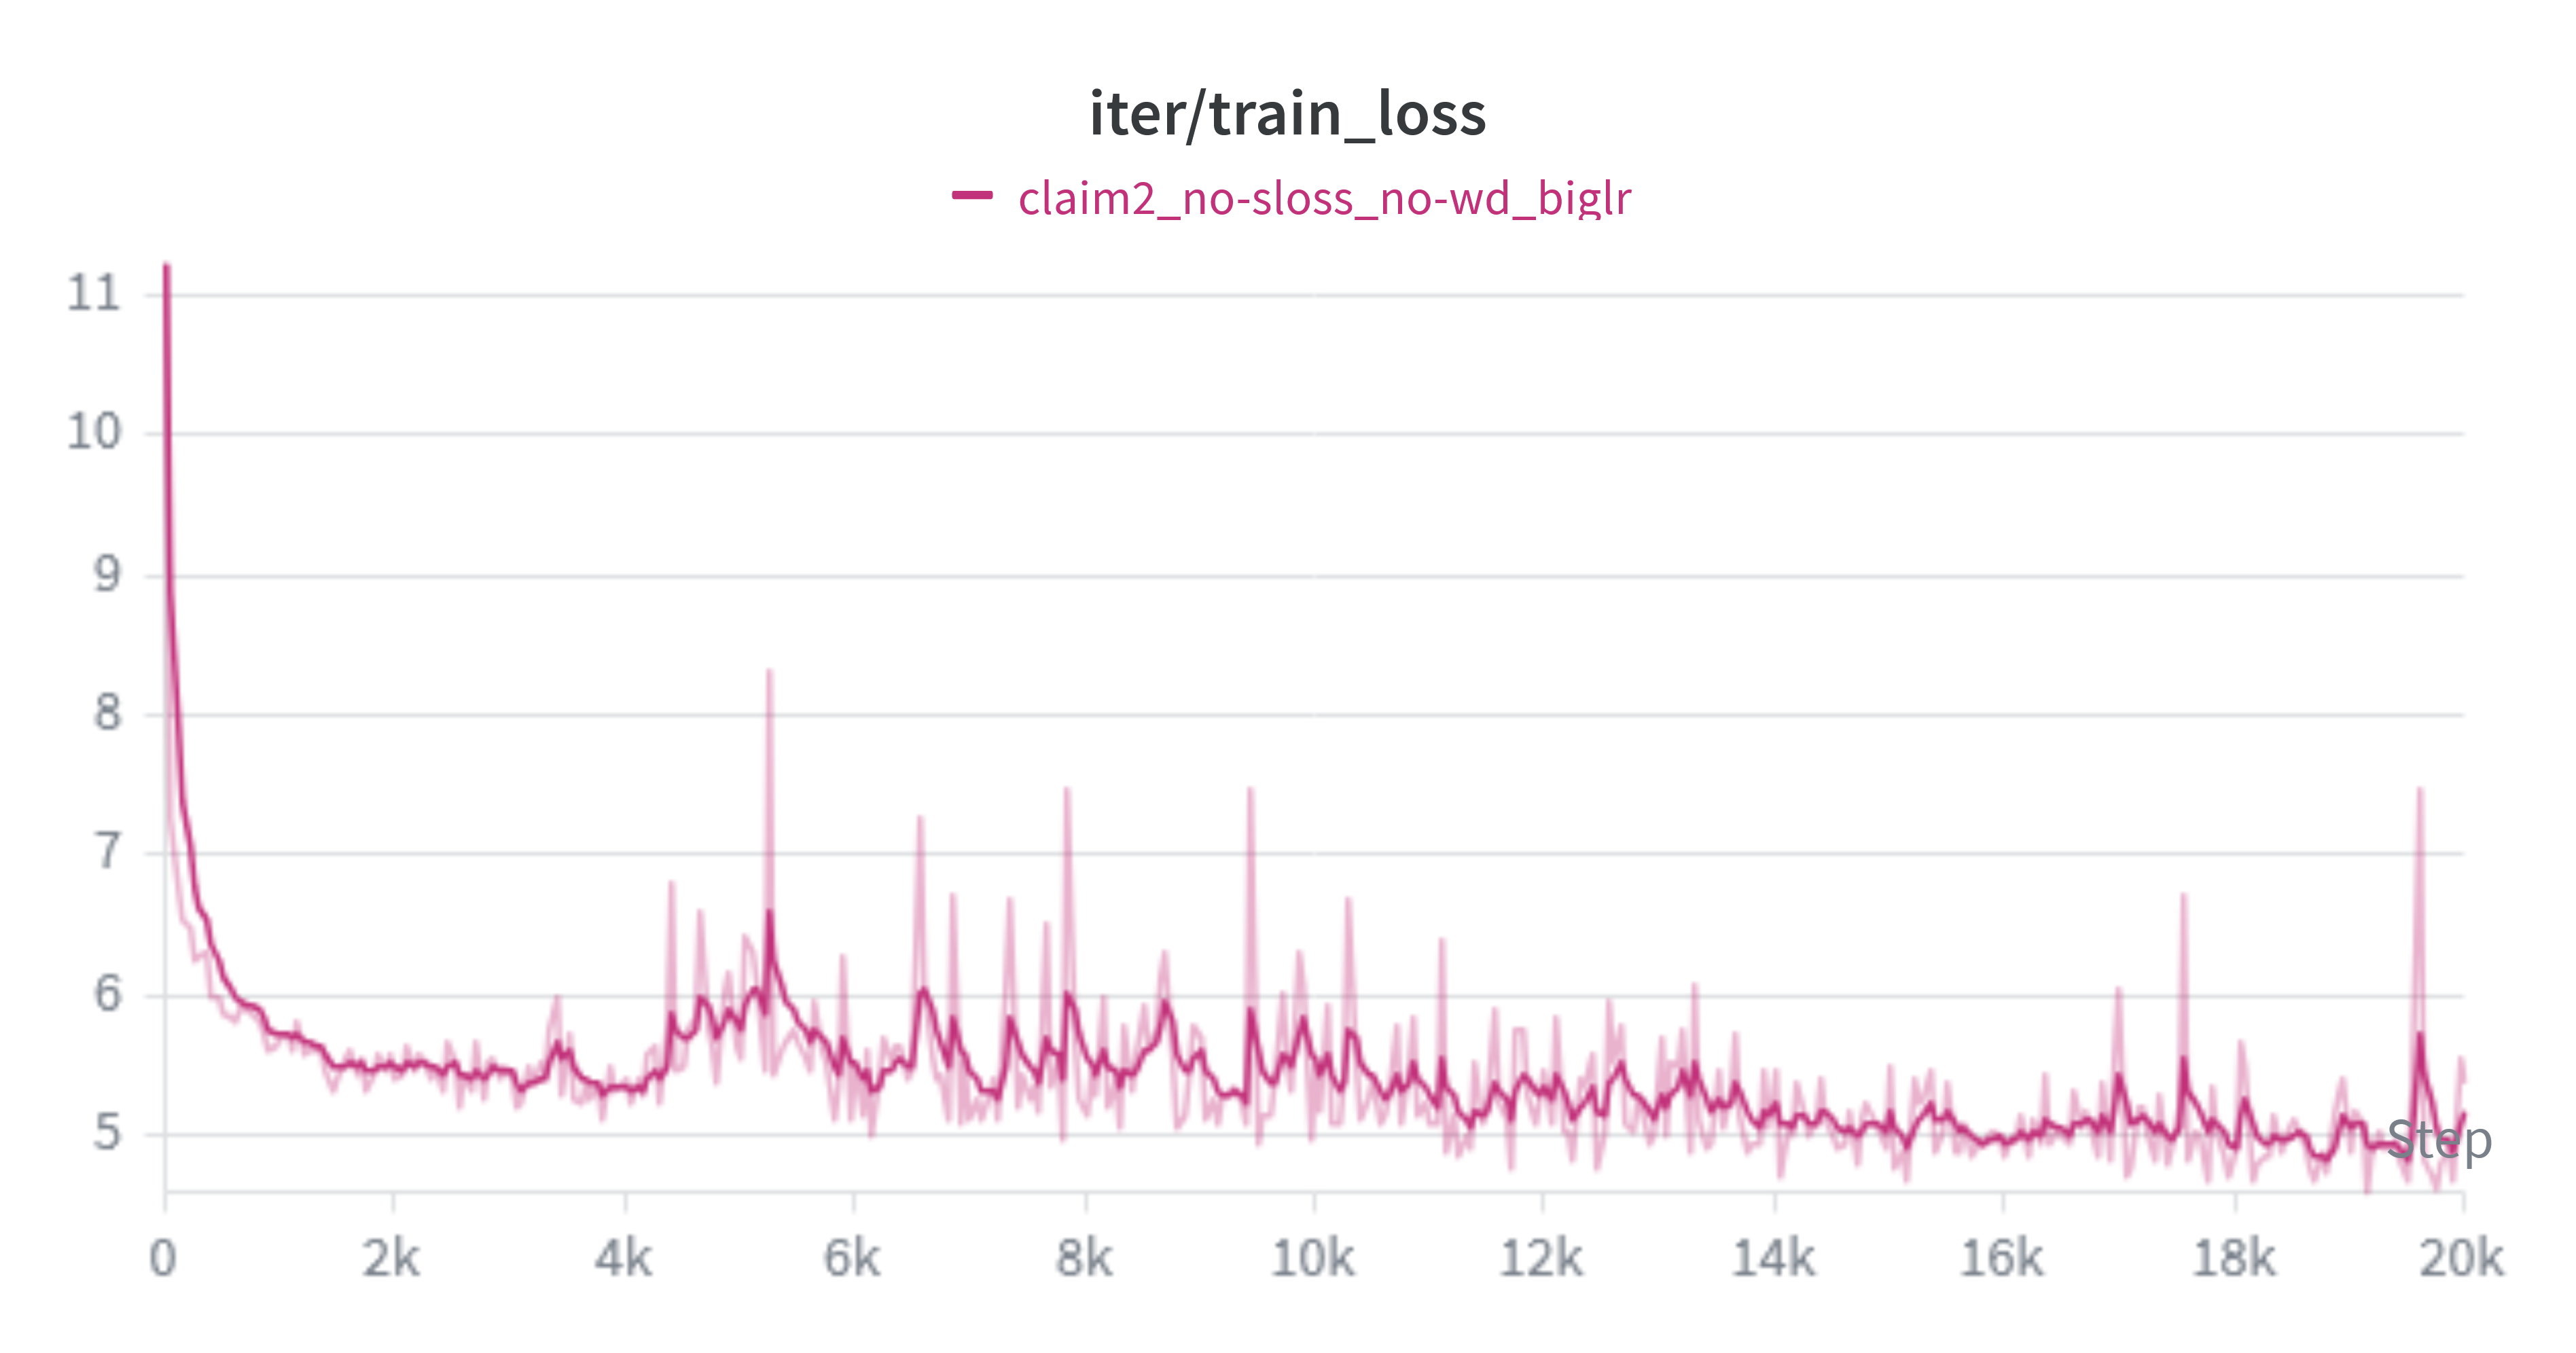
\includegraphics[width=\linewidth]{../rapport/figures/C2_train_loss_mehstable.png}
\end{minipage}
\hfill
\begin{minipage}{0.48\linewidth}
    \centering
    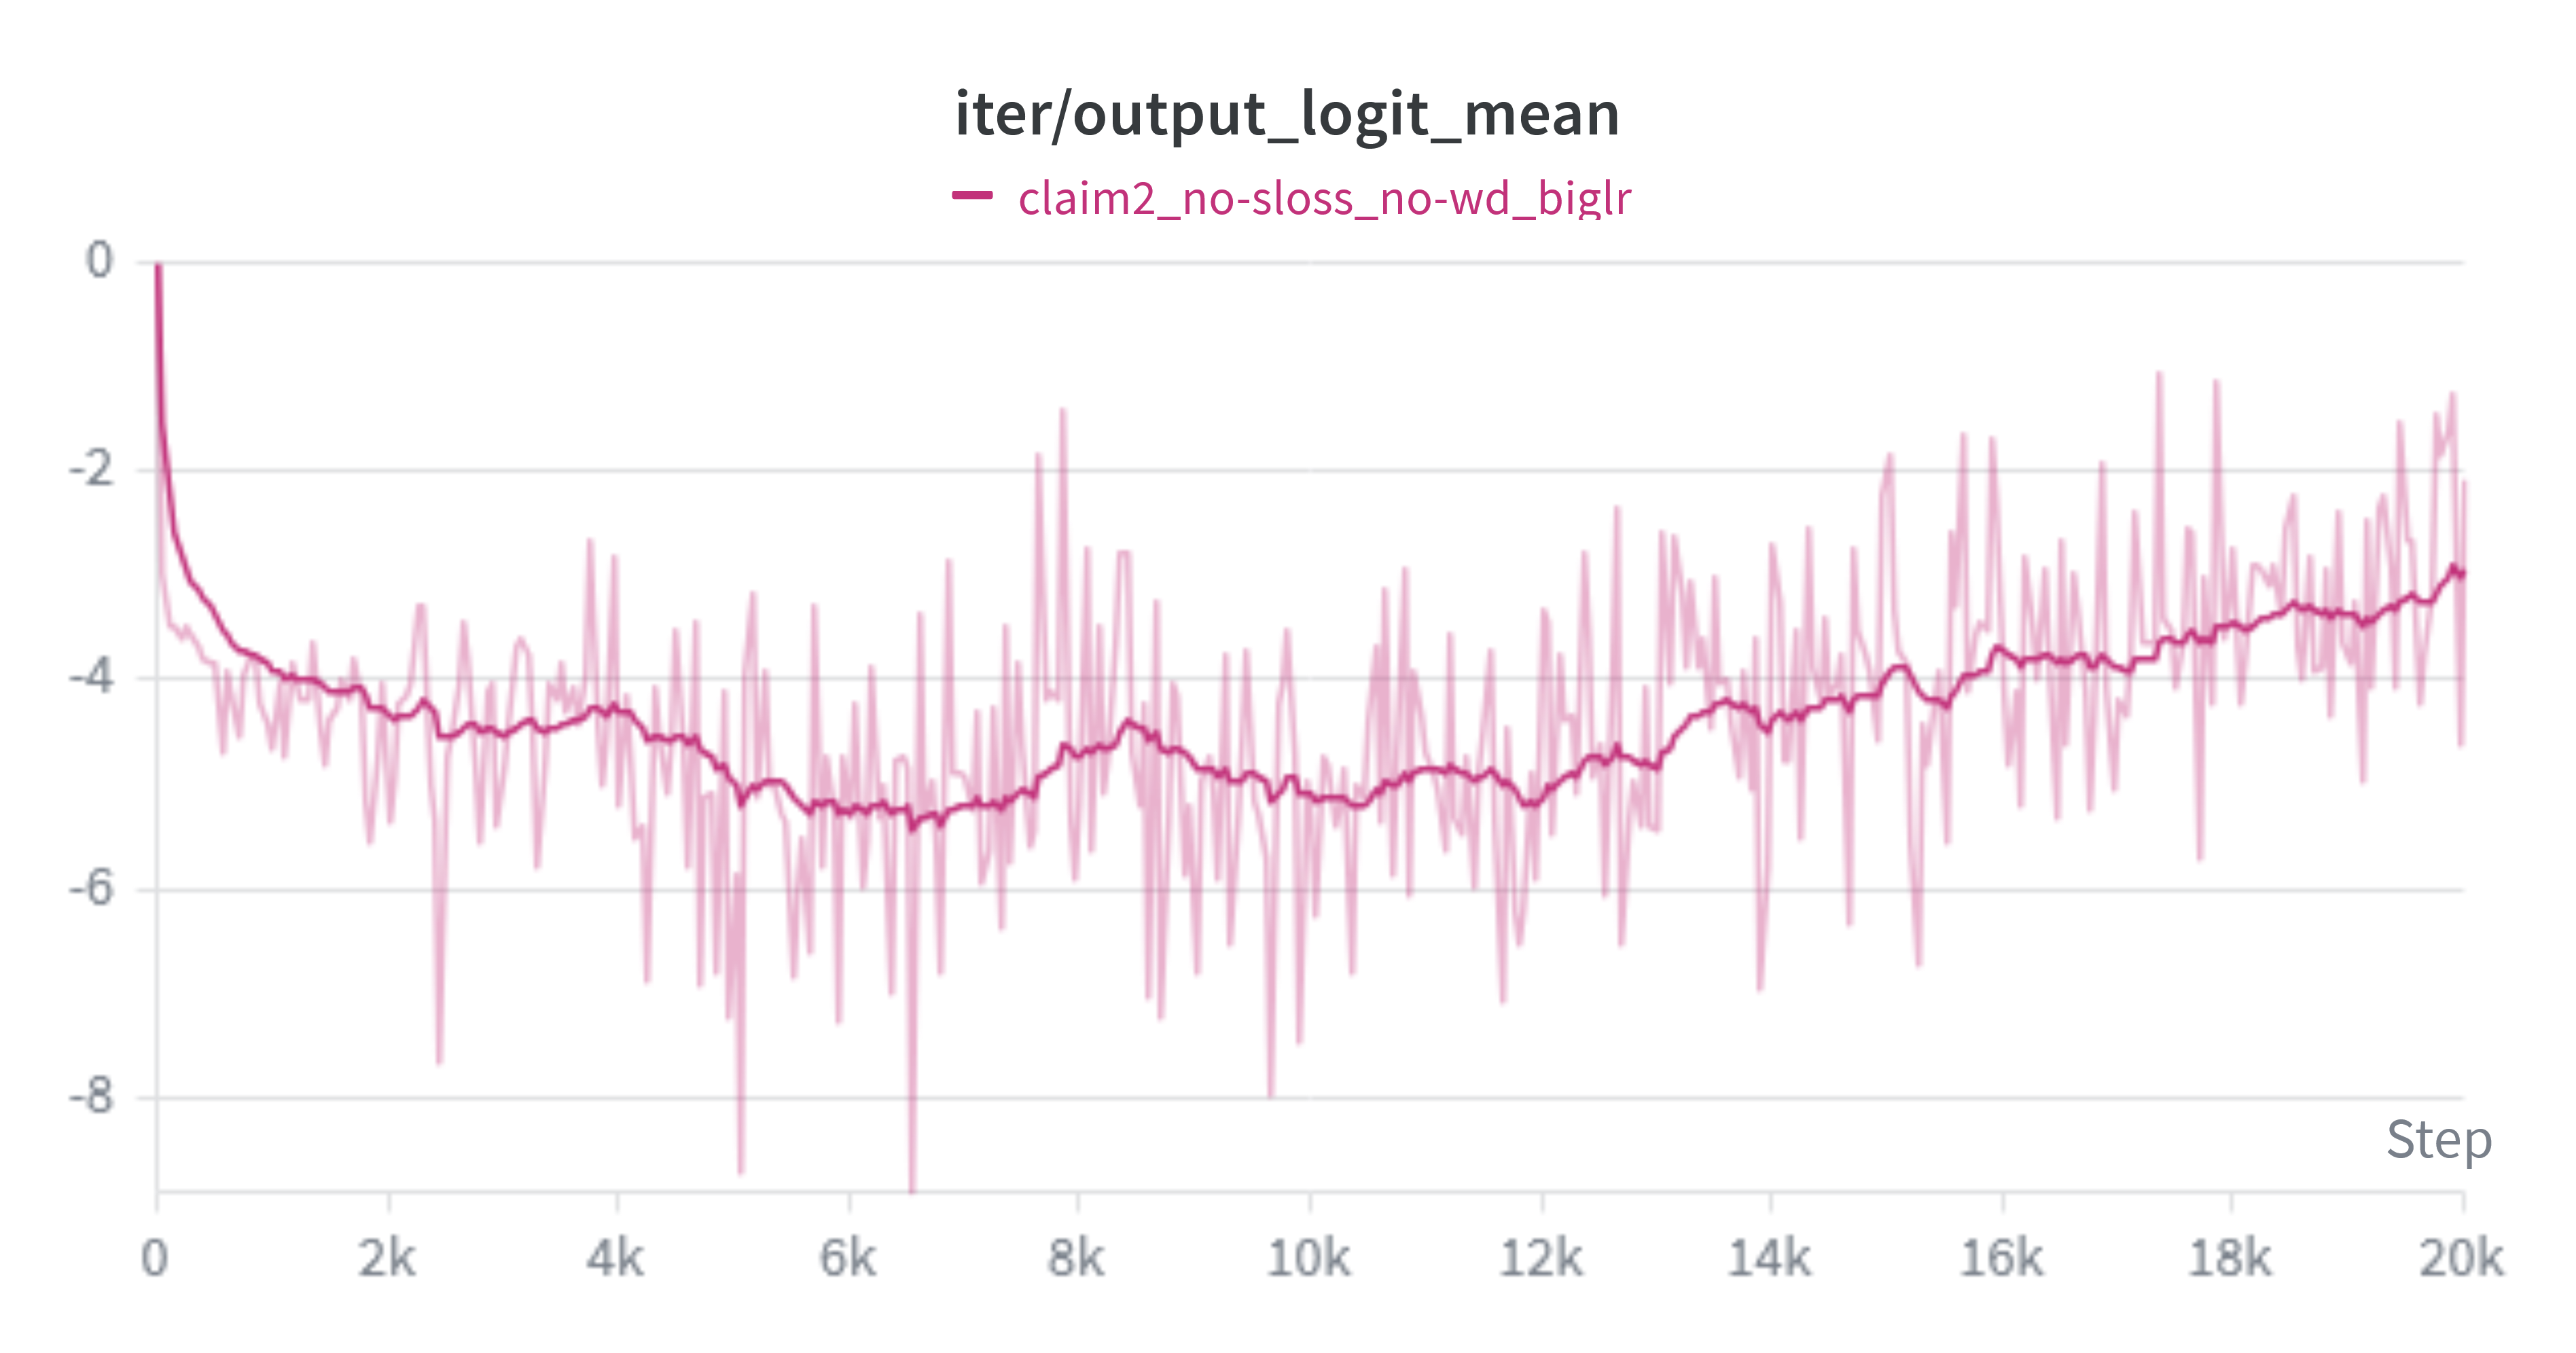
\includegraphics[width=\linewidth]{../rapport/figures/C2_mean_meh_stable.png}
\end{minipage}
\begin{minipage}{0.48\linewidth}
    \centering
    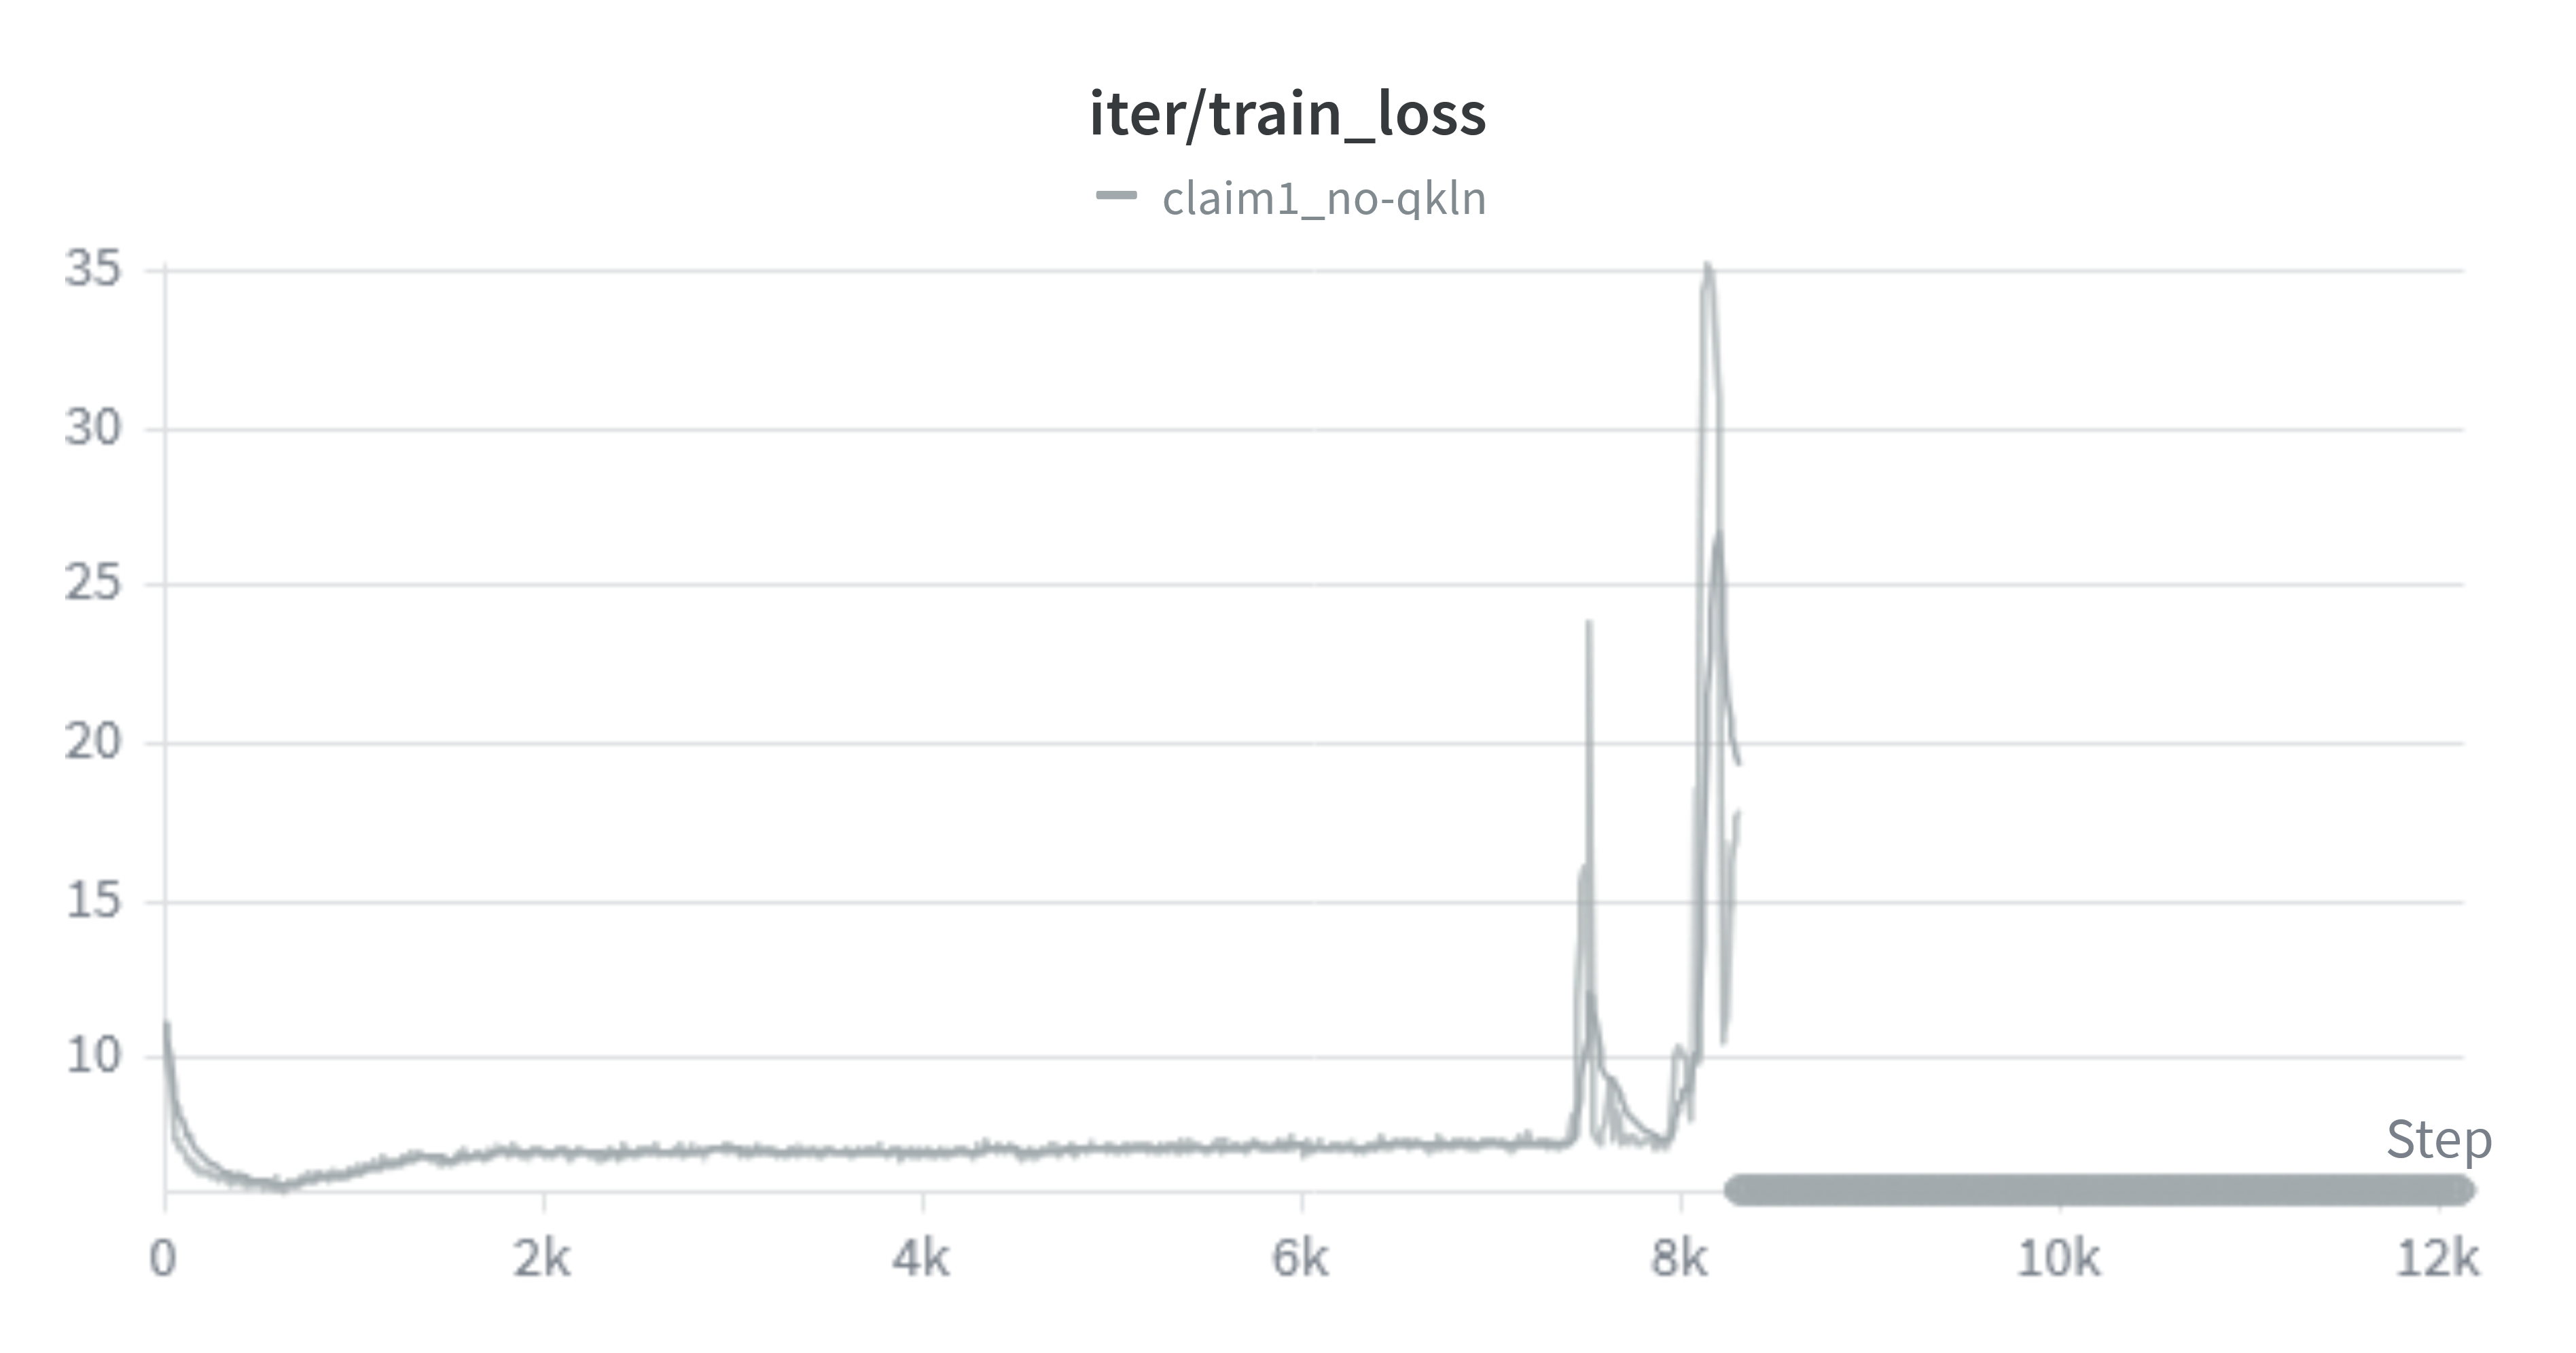
\includegraphics[width=\linewidth]{../rapport/figures/C2_train_unstable.png}
    
    {\footnotesize Unstable --- train loss}
\end{minipage}
\hfill
\begin{minipage}{0.48\linewidth}
    \centering
    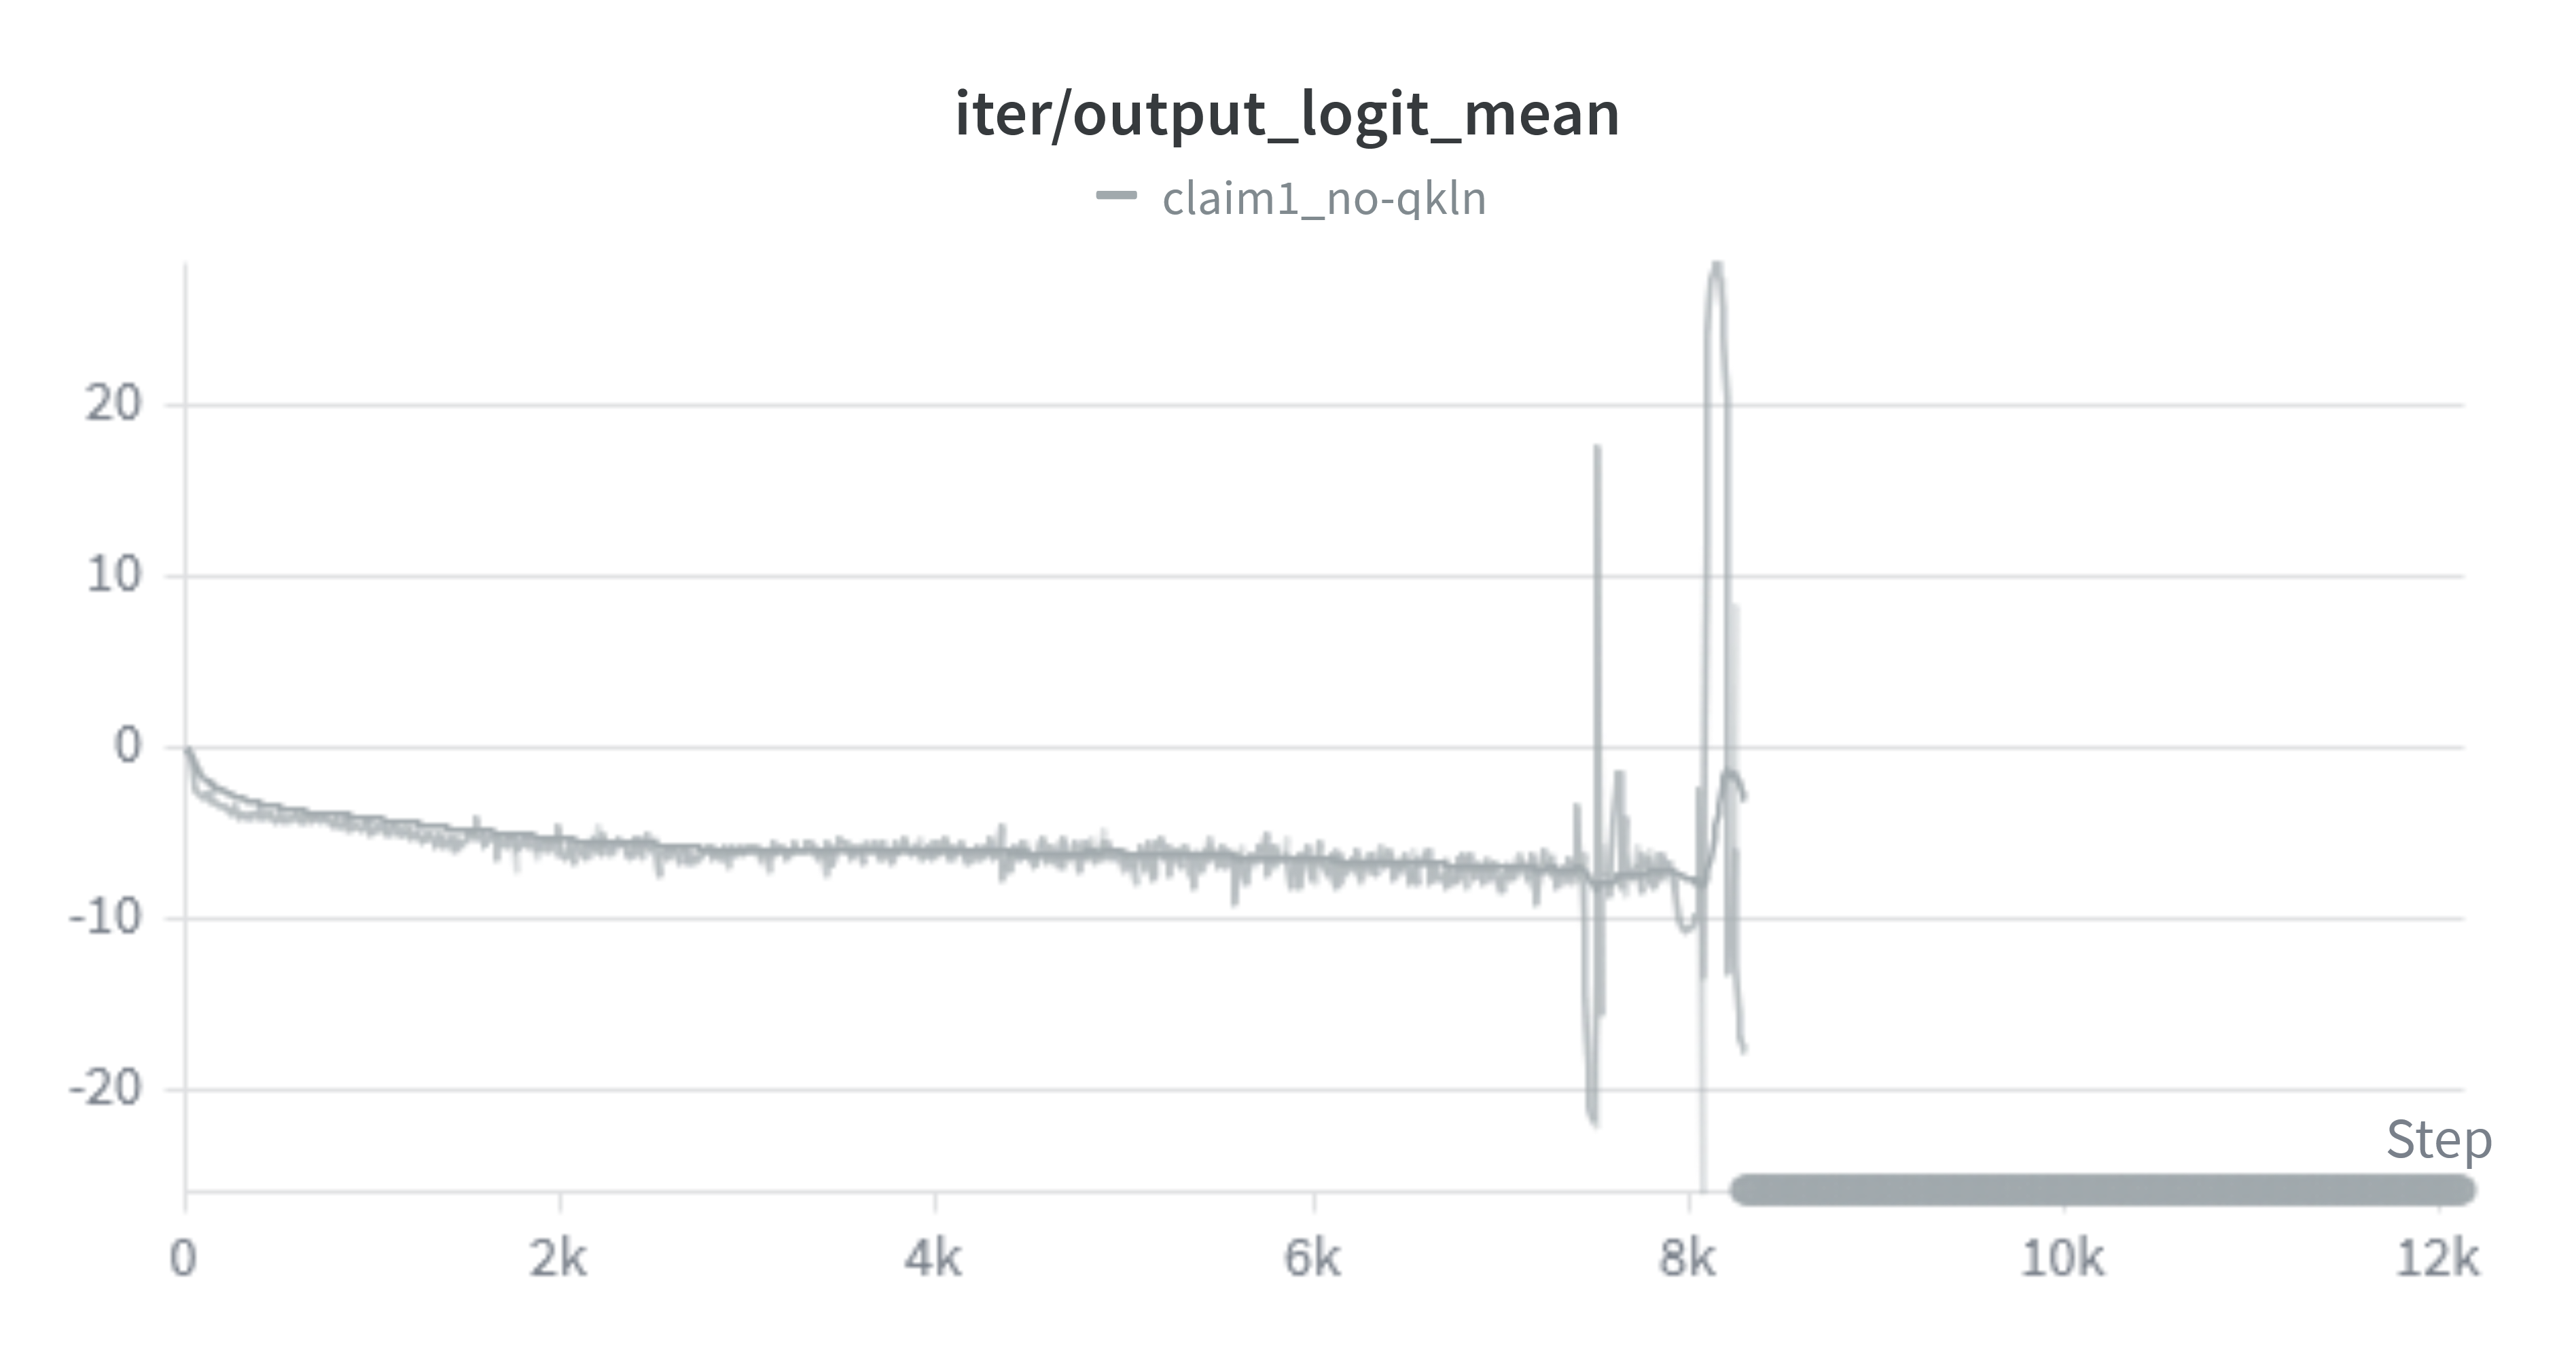
\includegraphics[width=\linewidth]{../rapport/figures/C2_mean_unstable.png}
    
    {\footnotesize Unstable --- logit mean}
\end{minipage}


{\footnotesize
\textbf{Claim 2 experiments across three regimes.}
Top: stable training run (\(lr=0.1\)).
Middle: moderately stable regime with mild fluctuations (linear warmup to \(lr=0.5\)).
Bottom: unstable regime showing divergence.
In all three cases, we did not observe a collapse of the output logit mean to \(-\infty\).
}
\newpage

% ══════════════════════════════════════════════════════════════════════════════
%  PAGE 4 — LR SENSITIVITY METRIC + FURTHER INSIGHTS + DISCUSSION
% ══════════════════════════════════════════════════════════════════════════════

\begin{tcolorbox}[
  enhanced, colback=successgreen!12, colframe=successgreen,
  arc=6pt, boxrule=1.5pt, left=10pt, right=10pt, top=6pt, bottom=6pt
]
  {\large\bfseries\color{successgreen} LR Sensitivity — A Unified Metric for Stability}
\end{tcolorbox}

\vspace{8pt}

\begin{multicols}{2}

\section{The LR Sensitivity Metric}

A model is \emph{fragile} if picking a slightly wrong learning rate leads to
significantly worse performance. The paper captures this with \textbf{LR Sensitivity}:

\[
\mathcal{S} = \mathbb{E}_{\eta \in [a,b]}\!\Bigl[\min\!\bigl(\ell(A(\eta)),\, \ell_0\bigr) - \ell^*\Bigr]
\]

\begin{itemize}[leftmargin=14pt, itemsep=2pt]
  \item $A(\eta)$ = model trained with learning rate $\eta$
  \item $\ell^* = \min_\eta \ell(A(\eta))$ = best achievable loss
  \item $\ell_0$ = loss at initialisation (caps diverged runs)
  \item Range $[a,b]$ spans \textbf{3 orders of magnitude}
\end{itemize}

\medskip
A high $\mathcal{S}$ means the model requires very careful LR tuning and is likely
to diverge if $\eta$ is even slightly too large.

\begin{claimbox}[Key finding]{successgreen}
\small
Both qk-layernorm and z-loss \textbf{reduce} $\mathcal{S}$. Models with these fixes
train stably across 3 orders of magnitude of LR variation. LR sensitivity still
\emph{increases with model scale}, but the mitigations slow this growth.
\end{claimbox}

\columnbreak

% Visual illustration of LR sensitivity concept
\begin{center}
\begin{tikzpicture}[font=\small]
  \draw[->] (0,0) -- (6.2,0) node[right] {\footnotesize LR ($\eta$)};
  \draw[->] (0,0) -- (0,4.5) node[above] {\footnotesize Final loss};

  % Fragile model curve
  \draw[alertred, very thick, smooth]
    plot[domain=0.3:5.8] (\x, {0.4*(\x-2)^2 + 1.2 + 1.5*max(0,\x-3.5)^1.8});
  \node[alertred, font=\footnotesize\bfseries] at (5.0, 4.0) {Fragile};
  \node[alertred, font=\footnotesize\bfseries] at (5.0, 3.7) {(high $\mathcal{S}$)};

  % Stable model curve
  \draw[successgreen, very thick, smooth]
    plot[domain=0.3:5.8] (\x, {0.1*(\x-2.5)^2 + 1.0});
  \node[successgreen, font=\footnotesize\bfseries] at (5.0, 1.9) {Stable};
  \node[successgreen, font=\footnotesize\bfseries] at (5.0, 1.6) {(low $\mathcal{S}$)};

  % Optimal marker
  \draw[dashed, medgray] (2.5, 0) -- (2.5, 1.0);
  \node[below, medgray, font=\footnotesize] at (2.5, 0) {$\eta^*$};

  % Annotation
  \draw[<->, thick, accentorange]
    (3.8, 2.3) -- (3.8, 3.8)
    node[midway, right, text width=1.4cm, font=\footnotesize, color=accentorange]
    {$\mathcal{S}$: area \\ above $\ell^*$};

  \node[font=\footnotesize\itshape, text width=5cm, align=center] at (3, -0.5)
    {The fragile model collapses if $\eta$ is slightly off};
\end{tikzpicture}
\end{center}

\end{multicols}

\vspace{6pt}

\section{Beyond the Two Instabilities — Paper Insights We Highlight}

\begin{multicols}{3}

\begin{graybox}[Warm-up reduces $\mathcal{S}$]
\small
Longer LR warm-up substantially reduces LR sensitivity, especially at large scale.
Models without warm-up cannot train stably at LR $3\times10^{-1}$, even with qk-layernorm.
\medskip

\textbf{Why it matters:} warm-up gives the adaptive optimizer time to build up reliable
moment estimates before committing to large gradient steps.
\end{graybox}

\columnbreak

\begin{graybox}[Depth $>$ Width for instability]
\small
Scaling \emph{depth} increases LR sensitivity \textbf{faster} than scaling width at
the same parameter count.

\medskip
However, the deepest models achieve the \emph{lowest} final loss, suggesting a
fundamental trade-off: depth buys performance but costs stability.
\end{graybox}

\columnbreak

\begin{graybox}[Predicting instability early]
\small
By tracking the \emph{max attention logit} as a function of model scale (fitted
with a quadratic), the paper \textbf{predicts} that a 4.8 B model will diverge at
LR $10^{-2}$ before running the experiment — and the prediction is confirmed.

\medskip
This is a powerful tool: identify failures \emph{cheaply} before they occur at scale.
\end{graybox}

\end{multicols}

% \vspace{6pt}
% \section{Discussion \& Lessons Learned}

% \begin{multicols}{2}

% \begin{claimbox}[What we successfully reproduced]{successgreen}
% \small
% \textbf{Claim 1 — Attention logit growth:} confirmed in our small-scale setup.
% The instability appears at high LR, max attention logits grow exponentially,
% and qk-layernorm fully prevents it. LR sensitivity is measurably reduced.
% The paper's central claim holds for this instability.
% \end{claimbox}

% \medskip
% \begin{claimbox}[What we could not reproduce]{alertred}
% \small
% \textbf{Claim 2 — Output logit divergence:} inconclusive. The specific failure mode
% (clean collapse of output logit mean to $-\infty$) was not observed in our setting.
% We either got stable training or global divergence, never the clean pattern shown
% in the paper's Figure 4.
% \end{claimbox}

% \columnbreak

% \begin{keybox}[Key Takeaways]
% \small
% \begin{enumerate}[leftmargin=14pt, itemsep=3pt]
%   \item Small-scale proxies \textbf{do work} for attention logit growth — this instability
%         is reliably elicited by high LR in models with $\sim$9 M parameters.

%   \item Reproducing output logit divergence is \textbf{more sensitive} to implementation
%         details than the paper suggests — dataset, warmup schedule, and exact optimizer
%         settings all seem to matter.

%   \item The LR sensitivity metric is a \textbf{useful diagnostic}: it clearly separates
%         stable from unstable configurations and tracks the effect of mitigations.

%   \item The \textbf{predict-then-confirm} methodology for instabilities is scientifically
%         compelling and opens a new paradigm for scaling studies.
% \end{enumerate}
% \end{keybox}

% \end{multicols}

% \vspace{6pt}

% \begin{tcolorbox}[
%   enhanced, colback=lightblue, colframe=midblue,
%   arc=4pt, boxrule=1pt, left=8pt, right=8pt, top=4pt, bottom=4pt
% ]
% \small
% \textbf{Broader impact:} This work shifts the paradigm for studying training instabilities —
% from ``wait for a large run to fail'' to ``reproduce cheaply, fix early, scale confidently.''
% The key tools — LR sensitivity measurement and high-LR small-scale proxies — are immediately
% practical for any team training large Transformers. The methodology also opens the door to
% \emph{proactive} instability detection via scaling trends of model characteristics.
% \end{tcolorbox}

\end{document}
